\chapter{导数和微分}

\section{导数的概念}

\subsection{导数的定义}

导数的思想最初是由法国数学家费马 (Fermat) 为研究极值问题而引入的, 但与导数概念直接相联系的是以下两个问题: 已知运动规律求速度和已知曲线求它的切线. 这是由英国数学家牛顿 (Newton) 和德国数学家莱布尼茨 (Leibniz) 分别在研究力学和几何学过程中建立起来的.

下面我们以这两个问题为背景引入导数的概念.

1. 瞬时速度 设一质点作直线运动,其运动规律为 \(s = s\left( t\right)\) . 若 \({t}_{0}\) 为某一确定的时刻, \(t\) 为邻近于 \({t}_{0}\) 的时刻,则
\[
\bar{v} = \frac{s\left( t\right)  - s\left( {t}_{0}\right) }{t - {t}_{0}}
\]
是质点在时间段 \(\left\lbrack  {{t}_{0},t}\right\rbrack\) (或 \(\left\lbrack  {t,{t}_{0}}\right\rbrack\) ) 上的平均速度. 若 \(t \rightarrow  {t}_{0}\) 时平均速度 \(\bar{v}\) 的极限存在,则称极限
\[
v = \mathop{\lim }\limits_{{t \rightarrow  {t}_{0}}}\frac{s\left( t\right)  - s\left( {t}_{0}\right) }{t - {t}_{0}} \tag{1}
\]
为质点在时刻 \({t}_{0}\) 的瞬时速度. 以后我们将会发现,在计算诸如物质比热、电流强度、线密度等问题中, 尽管它们的物理背景各不相同, 但最终都归结于讨论形如 (1) 式的极限.

2. 切线的斜率 如图 5-1 所示,曲线 \(y = f\left( x\right)\) 在其上一点 \(P\left( {{x}_{0},{y}_{0}}\right)\) 处的切线 \({PT}\) 是割线 \({PQ}\) 当动点 \(Q\) 沿此曲线无限接近于点 \(P\) 时的极限位置. 由于割线 \({PQ}\) 的斜率为
\[
\bar{k} = \frac{f\left( x\right)  - f\left( {x}_{0}\right) }{x - {x}_{0}},
\]
\begin{figure}
	\centering
	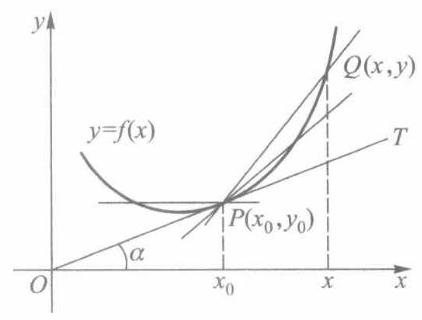
\includegraphics[width=.3\textwidth]{images/P022.jpg}
	\caption{图 $5-1$}
	\label{fig:P022}
\end{figure}

因此当 \(x \rightarrow  {x}_{0}\) 时,如果 \(\bar{k}\) 的极限存在,则极限
\[
k = \mathop{\lim }\limits_{{x \rightarrow  {x}_{0}}}\frac{f\left( x\right)  - f\left( {x}_{0}\right) }{x - {x}_{0}} \tag{2}
\]
即为切线 \({PT}\) 的斜率.

上述两个问题中, 前一个是运动学的问题, 后一个是几何学的问题, 但是它们都可以归结为形如 \(\left( 1\right) \text{ 、 }\left( 2\right)\) 这种类型的极限.

下面我们给出导数的定义.

%定义  1
\begin{definition}{导数}{def:导数}
设函数 \(y = f\left( x\right)\) 在点 \({x}_{0}\) 的某邻域内有定义,若极限
\[
\mathop{\lim }\limits_{{x \rightarrow  {x}_{0}}}\frac{f\left( x\right)  - f\left( {x}_{0}\right) }{x - {x}_{0}} \tag{3}
\]
存在,则称函数 \(f\) 在点 \({x}_{0}\) 可导,并称该极限为函数 \(f\) 在点 \({x}_{0}\) 的导数,记作 \({f}^{\prime }\left( {x}_{0}\right)\) .
\end{definition}


令 \(x = {x}_{0} + {\Delta x},{\Delta y} = f\left( {{x}_{0} + {\Delta x}}\right)  - f\left( {x}_{0}\right)\) ,则 (3) 式可改写为
\[
\mathop{\lim }\limits_{{{\Delta x} \rightarrow  0}}\frac{\Delta y}{\Delta x} = \mathop{\lim }\limits_{{{\Delta x} \rightarrow  0}}\frac{f\left( {{x}_{0} + {\Delta x}}\right)  - f\left( {x}_{0}\right) }{\Delta x} = {f}^{\prime }\left( {x}_{0}\right) . \tag{4}
\]
所以导数是函数增量 \({\Delta y}\) 与自变量增量 \({\Delta x}\) 之比 \(\frac{\Delta y}{\Delta x}\) 的极限. 这个增量比称为函数关于自变量的平均变化率 (又称差商),而导数 \({f}^{\prime }\left( {x}_{0}\right)\) 则为 \(f\) 在 \({x}_{0}\) 处关于 \(x\) 的变化率.

若 (3) (或 (4))式极限不存在,则称 \(f\) 在点 \({x}_{0}\) 不可导.

%例 1
\begin{example}
求函数 \(f\left( x\right)  = {x}^{2}\) 在点 \(x = 1\) 的导数,并求曲线在点(1,1)的切线方程.
\end{example}


%解
\begin{solution}
由定义求得
\[
{f}^{\prime }\left( 1\right)  = \mathop{\lim }\limits_{{{\Delta x} \rightarrow  0}}\frac{f\left( {1 + {\Delta x}}\right)  - f\left( 1\right) }{\Delta x} = \mathop{\lim }\limits_{{{\Delta x} \rightarrow  0}}\frac{{\left( 1 + \Delta x\right) }^{2} - 1}{\Delta x}
\]
\[
= \mathop{\lim }\limits_{{{\Delta x} \rightarrow  0}}\frac{{2\Delta x} + \Delta {x}^{2}}{\Delta x} = \mathop{\lim }\limits_{{{\Delta x} \rightarrow  0}}\left( {2 + {\Delta x}}\right)  = 2.
\]
由此知道抛物线 \(y = {x}^{2}\) 在点(1,1)的切线斜率为
\[
k = {f}^{\prime }\left( 1\right)  = 2,
\]
所以切线方程为
\[
y - 1 = 2\left( {x - 1}\right) \text{ 即 }y = {2x} - 1.
\]
\end{solution}

%例 2
\begin{example}
证明函数 \(f\left( x\right)  = \left| x\right|\) 在点 \({x}_{0} = 0\) 不可导.
\end{example}


%证
\begin{proof}
因为
\[
\frac{f\left( x\right)  - f\left( 0\right) }{x - 0} = \frac{\left| x\right| }{x} = \left\{  \begin{matrix} 1, & x > 0, \\   - 1, & x < 0 \end{matrix}\right.
\]
当 \(x \rightarrow  0\) 时极限不存在,所以 \(f\) 在点 \(x = 0\) 不可导.
\end{proof}


%例 3
\begin{example}
显然常量函数 \(f\left( x\right)  = C\) 在任何一点 \(x\) 的导数都等于零,即
\[
{f}^{\prime }\left( x\right)  = 0.
\]
\end{example}

下面我们介绍有限增量公式.

设 \(f\left( x\right)\) 在点 \({x}_{0}\) 可导,那么
\[
\varepsilon  = \frac{\Delta y}{\Delta x} - {f}^{\prime }\left( {x}_{0}\right)
\]
是当 \({\Delta x} \rightarrow  0\) 时的无穷小量,于是 \(\varepsilon  \cdot  {\Delta x} = o\left( {\Delta x}\right)\) ,即
\[
{\Delta y} = {f}^{\prime }\left( {x}_{0}\right) {\Delta x} + o\left( {\Delta x}\right) . \tag{5}
\]
我们称 (5) 式为 \(f\left( x\right)\) 在点 \({x}_{0}\) 的有限增量公式. 注意,此公式对 \({\Delta x} = 0\) 仍旧成立.

由公式 (5) 立即推得如下定理.

%定理 5.1
\begin{theorem}{可导与连续}{the:可导与连续}
若函数 \(f\) 在点 \({x}_{0}\) 可导,则 \(f\) 在点 \({x}_{0}\) 连续.
\end{theorem}


%注
\begin{remark}
可导仅是函数在该点连续的充分条件, 而不是必要条件. 如例 2 中的函数 \(f\left( x\right)  = \left| x\right|\) 在点 \(x = 0\) 连续,但不可导.

\end{remark}

%例 4
\begin{example}
证明函数 \(f\left( x\right)  = {x}^{2}D\left( x\right)\) 仅在点 \({x}_{0} = 0\) 可导,其中 \(D\left( x\right)\) 为狄利克雷函数.
\end{example}


%证
\begin{proof}
当 \({x}_{0} \neq  0\) 时,由归结原则可得 \(f\left( x\right)\) 在点 \(x = {x}_{0}\) 不连续,所以由定理 5.1, \(f\left( x\right)\) 在点 \(x = {x}_{0}\) 不可导.

当 \({x}_{0} = 0\) 时,由于 \(D\left( x\right)\) 为有界函数,因此得到
\[
{f}^{\prime }\left( 0\right)  = \mathop{\lim }\limits_{{x \rightarrow  0}}\frac{f\left( x\right)  - f\left( 0\right) }{x - 0} = \mathop{\lim }\limits_{{x \rightarrow  0}}{xD}\left( x\right)  = 0.
\]
\end{proof}

若只讨论函数在点 \({x}_{0}\) 的右邻域 (左邻域) 上的变化率,我们需引进单侧导数的概念.

%定义  2
\begin{definition}{单侧导数}{def:单侧导数}
设函数 \(y = f\left( x\right)\) 在点 \({x}_{0}\) 的某右邻域 \(\left\lbrack  {{x}_{0},{x}_{0} + \delta }\right)\) 上有定义,若右极限
\[
\mathop{\lim }\limits_{{{\Delta x} \rightarrow  {0}^{ + }}}\frac{\Delta y}{\Delta x} = \mathop{\lim }\limits_{{{\Delta x} \rightarrow  {0}^{ + }}}\frac{f\left( {{x}_{0} + {\Delta x}}\right)  - f\left( {x}_{0}\right) }{\Delta x}\;\left( {0 < {\Delta x} < \delta }\right)
\]
存在,则称该极限值为 \(f\) 在点 \({x}_{0}\) 的右导数,记作 \({f}^{\prime }\left( {x}_{0}\right)\) .

类似地, 我们可定义左导数
\[
{f}^{\prime } - \left( {x}_{0}\right)  = \mathop{\lim }\limits_{{{\Delta x} \rightarrow  {0}^{ - }}}\frac{f\left( {{x}_{0} + {\Delta x}}\right)  - f\left( {x}_{0}\right) }{\Delta x}.
\]
右导数和左导数统称为单侧导数.
\end{definition}


如同左、右极限与极限之间的关系, 我们有

%定理 5.2
\begin{theorem}{可导条件}{the:可导条件}
若函数 \(y = f\left( x\right)\) 在点 \({x}_{0}\) 的某邻域上有定义,则 \({f}^{\prime }\left( {x}_{0}\right)\) 存在的充要条件是 \({f}_{ + }^{\prime }\left( {x}_{0}\right)\) 与 \({f}_{ - }^{\prime }\left( {x}_{0}\right)\) 都存在,且
\[
{f}^{\prime } + \left( {x}_{0}\right)  = {f}^{\prime } - \left( {x}_{0}\right) .
\]
\end{theorem}

%例 5
\begin{example}
设 \(f\left( x\right)  = \left\{  \begin{array}{ll} 1 - \cos x, & x \geq  0, \\  x, & x < 0. \end{array}\right.\) 讨论 \(f\left( x\right)\) 在点 \(x = 0\) 的左、右导数与导数.
\end{example}


%解
\begin{solution}
由于
\[
\frac{f\left( {0 + {\Delta x}}\right)  - f\left( 0\right) }{\Delta x} = \left\{  \begin{array}{ll} \frac{1 - \cos {\Delta x}}{\Delta x}, & {\Delta x} > 0, \\  1, & {\Delta x} < 0, \end{array}\right.
\]
因此
\[
{f}_{ + }^{\prime }\left( 0\right)  = \mathop{\lim }\limits_{{{\Delta x} \rightarrow  {0}^{ + }}}\frac{1 - \cos {\Delta x}}{\Delta x} = 0,
\]
\[
{f}_{ - }^{\prime }\left( 0\right)  = \mathop{\lim }\limits_{{{\Delta x} \rightarrow  {0}^{ - }}}1 = 1.
\]
因为 \({f}^{\prime }{}_{ + }\left( 0\right)  \neq  {f}^{\prime }{}_{ - }\left( 0\right)\) ,所以 \(f\) 在点 \(x = 0\) 不可导.
\end{solution}

\subsection{导函数}

若函数在区间 \(I\) 上每一点都可导 (对区间端点,仅考虑相应的单侧导数),则称 \(f\) 为 \(I\) 上的可导函数. 此时对每一个 \(x \in  I\) ,都有 \(f\) 的一个导数 \({f}^{\prime }\left( x\right)\) (或单侧导数) 与之对应. 这样就定义了一个在 \(I\) 上的函数,称为 \(f\) 在 \(I\) 上的导函数,也简称为导数. 记作 \({f}^{\prime },{y}^{\prime }\) 或 \(\frac{\mathrm{d}y}{\mathrm{\;d}x}\) ,即
\[
{f}^{\prime }\left( x\right)  = \mathop{\lim }\limits_{{{\Delta x} \rightarrow  0}}\frac{f\left( {x + {\Delta x}}\right)  - f\left( x\right) }{\Delta x},\;x \in  I.
\]
在物理学中,导数 \({y}^{\prime }\) 也常用牛顿记号 \(\dot{y}\) 表示,而记号 \(\frac{\mathrm{d}y}{\mathrm{\;d}x}\) 是莱布尼茨首先引用的. 目前我们把 \(\frac{\mathrm{d}y}{\mathrm{\;d}x}\) 看作一个整体,也可把它理解为 \(\frac{\mathrm{d}}{\mathrm{d}x}\) 施加于 \(y\) 的求导运算,待到学过 “微分” 之后,我们将说明这个记号实际上是一个“商”. 相应于上述各种表示导数的形式, \({f}^{\prime }\left( {x}_{0}\right)\) 有时也写作
\[
{\left. {y}^{\prime }\right| }_{x = {x}_{0}}\text{ 或 }{\left. \frac{\mathrm{d}y}{\mathrm{\;d}x}\right| }_{x = {x}_{0}}.
\]
%例 6
\begin{example}
证明

(i) \({\left( {x}^{n}\right) }^{\prime } = n{x}^{n - 1},n\) 为正整数;

(ii) \({\left( \sin x\right) }^{\prime } = \cos x,{\left( \cos x\right) }^{\prime } =  - \sin x\) ;

(iii) \({\left( {\log }_{a}x\right) }^{\prime } = \frac{1}{x}{\log }_{a}\mathrm{e}\left( {a > 0,a \neq  1,x > 0}\right)\) ,特别 \({\left( \ln x\right) }^{\prime } = \frac{1}{x}\) .
\end{example}


%证
\begin{proof}
(i) 对于 \(y = {x}^{n}\) ,由于
\[
\frac{\Delta y}{\Delta x} = \frac{{\left( x + \Delta x\right) }^{n} - {x}^{n}}{\Delta x} = {\mathrm{C}}_{n}^{1}{x}^{n - 1} + {\mathrm{C}}_{n}^{2}{x}^{n - 2}{\Delta x} + \cdots  + {\mathrm{C}}_{n}^{n}\Delta {x}^{n - 1},
\]
因此
\[
{y}^{\prime } = \mathop{\lim }\limits_{{{\Delta x} \rightarrow  0}}\frac{\Delta y}{\Delta x} = \mathop{\lim }\limits_{{{\Delta x} \rightarrow  0}}\left( {{\mathrm{C}}_{n}^{1}{x}^{n - 1} + {\mathrm{C}}_{n}^{2}{x}^{n - 2}{\Delta x} + \cdots  + {\mathrm{C}}_{n}^{n}\Delta {x}^{n - 1}}\right)  = {\mathrm{C}}_{n}^{1}{x}^{n - 1} = n{x}^{n - 1}.
\]
(ii) 下面证第一个等式, 类似地可证第二个等式. 由于
\[
\frac{\sin \left( {x + {\Delta x}}\right)  - \sin x}{\Delta x} = \frac{2\sin \frac{\Delta x}{2}\cos \left( {x + \frac{\Delta x}{2}}\right) }{\Delta x} = \frac{\sin \frac{\Delta x}{2}}{\frac{\Delta x}{2}}\cos \left( {x + \frac{\Delta x}{2}}\right) ,
\]
以及 \(\cos x\) 是 \(\left( {-\infty , + \infty }\right)\) 上的连续函数,因此得到
\[
{\left( \sin x\right) }^{\prime } = \mathop{\lim }\limits_{{{\Delta x} \rightarrow  0}}\frac{\sin \frac{\Delta x}{2}}{\frac{\Delta x}{2}} \cdot  \mathop{\lim }\limits_{{{\Delta x} \rightarrow  0}}\cos \left( {x + \frac{\Delta x}{2}}\right)  = \cos x.
\]
(iii) 由于
\[
\frac{{\log }_{a}\left( {x + {\Delta x}}\right)  - {\log }_{a}x}{\Delta x} = \frac{1}{\Delta x}{\log }_{a}\left( {1 + \frac{\Delta x}{x}}\right)  = \frac{1}{x}{\log }_{a}{\left( 1 + \frac{\Delta x}{x}\right) }^{\frac{x}{\Delta x}},
\]
所以
\[
{\left( {\log }_{a}x\right) }^{\prime } = \mathop{\lim }\limits_{{{\Delta x} \rightarrow  0}}\frac{1}{x}{\log }_{a}{\left( 1 + \frac{\Delta x}{x}\right) }^{\frac{x}{\Delta x}} = \frac{1}{x}{\log }_{a}\mathrm{e}. \tag{6}
\]
\end{proof}

若 \(a = \mathrm{e}\) ,且以 \(\mathrm{e}\) 为底的自然对数常写作 \(\ln x\) ,则由 \(\ln \mathrm{e} = 1\) 及 (6) 式有
\[
{\left( \ln x\right) }^{\prime } = \frac{1}{x}.
\]
\subsection{导数的几何意义}

我们已经知道 \(f\left( x\right)\) 在点 \(x = {x}_{0}\) 的切线斜率 \(k\) ,正是割线斜率在 \(x \rightarrow  {x}_{0}\) 时的极限, 即
\[
k = \mathop{\lim }\limits_{{x \rightarrow  {x}_{0}}}\frac{f\left( x\right)  - f\left( {x}_{0}\right) }{x - {x}_{0}}.
\]
由导数的定义, \(k = {f}^{\prime }\left( {x}_{0}\right)\) ,所以曲线 \(y = f\left( x\right)\) 在点 \(\left( {{x}_{0},{y}_{0}}\right)\) 的切线方程是
\[
y - {y}_{0} = {f}^{\prime }\left( {x}_{0}\right) \left( {x - {x}_{0}}\right) . \tag{7}
\]
这就是说: 函数 \(f\) 在点 \({x}_{0}\) 的导数 \({f}^{\prime }\left( {x}_{0}\right)\) 是曲线 \(y = f\left( x\right)\) 在点 \(\left( {{x}_{0},{y}_{0}}\right)\) 的切线斜率. 若 \(\alpha\) 表示这条切线与 \(x\) 轴正向的夹角,则 \({f}^{\prime }\left( {x}_{0}\right)  = \tan \alpha\) . 从而 \({f}^{\prime }\left( {x}_{0}\right)  > 0\) 意味着切线与 \(x\) 轴正向的夹角为锐角; \({f}^{\prime }\left( {x}_{0}\right)  < 0\) 意味着切线与 \(x\) 轴正向的夹角为钝角; \({f}^{\prime }\left( {x}_{0}\right)  = 0\) 表示切线与 \(x\) 轴平行 (图 5-2).

\begin{figure}
	\centering
	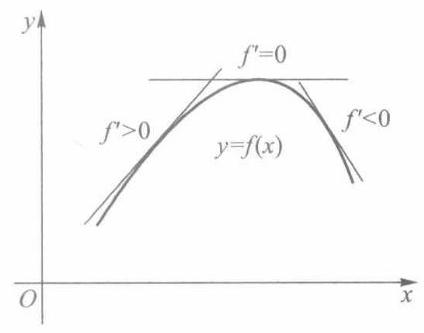
\includegraphics[width=.3\textwidth]{images/P023.jpg}
	\caption{图 $5-2$}
	\label{fig:P023}
\end{figure}

%例 7
\begin{example}
求曲线 \(y = {x}^{3}\) 在点 \(P\left( {{x}_{0},{y}_{0}}\right)\) 的切线方程与法线方程.
\end{example}


%解
\begin{solution}
由于
\[
\frac{\Delta y}{\Delta x} = 3{x}_{0}^{2} + 3{x}_{0}{\Delta x} + \Delta {x}^{2},
\]
\[
{f}^{\prime }\left( {x}_{0}\right)  = \mathop{\lim }\limits_{{{\Delta x} \rightarrow  0}}\left( {3{x}_{0}^{2} + 3{x}_{0}{\Delta x} + \Delta {x}^{2}}\right)  = 3{x}_{0}^{2}.
\]
所以根据 (7) 式,曲线 \(y = {x}^{3}\) 在点 \(P\) 的切线方程为
\[
y - {y}_{0} = 3{x}_{0}^{2}\left( {x - {x}_{0}}\right) .
\]
由解析几何知道,若切线斜率为 \(k\) ,则法线斜率为 \(- \frac{1}{k}\) . 从而过点 \(P\) 的法线方程为
\[
y - {y}_{0} =  - \frac{1}{{f}^{\prime }\left( {x}_{0}\right) }\left( {x - {x}_{0}}\right) . \tag{8}
\]
\end{solution}

因此曲线 \(y = {x}^{3}\) 过点 \(P\left( {{x}_{0} \neq  0}\right)\) 的法线方程为
\[
y - {x}_{0}^{3} =  - \frac{1}{3{x}_{0}^{2}}\left( {x - {x}_{0}}\right) .
\]
若 \({x}_{0} = 0\) ,则法线方程为 \(x = 0\) .

顺便说一下,对于曲线 \(y = {x}^{3}\) ,可把它在点 \(P\left( {{x}_{0},{y}_{0}}\right)\) 的切线斜率 \({f}^{\prime }\left( {x}_{0}\right)\) 改写成如下形式:
\[
{f}^{\prime }\left( {x}_{0}\right)  = 3{x}_{0}^{2} = \frac{{x}_{0}^{3}}{\frac{{x}_{0}}{3}} = \frac{{y}_{0}}{\frac{{x}_{0}}{3}}.
\]
因此,为了作过点 \(P\) 的切线,如图 5-3 所示,只需对 \(x\) 轴上从原点 \(O\) 到点 \({x}_{0}\) 的线段三等分,取靠近 \({x}_{0}\) 的分点 \(Q\) ,那么直线 \({PQ}\) 就是所求的切线.

%定义  3
\begin{definition}{}{def:}
若函数 \(f\) 在点 \({x}_{0}\) 的某邻域 \(U\left( {x}_{0}\right)\) 上对一切 \(x \in  U\left( {x}_{0}\right)\) 有
\[
f\left( {x}_{0}\right)  \geq  f\left( x\right) \;\left( {f\left( {x}_{0}\right)  \leq  f\left( x\right) }\right) , \tag{9}
\]
\end{definition}

则称函数 \(f\) 在点 \({x}_{0}\) 取得极大 (小) 值,称点 \({x}_{0}\) 为极大 (小) 值点. 极大值、极小值统称为极值, 极大值点、极小值点统称为极值点.

设函数 \(f\) 如图 5-4 所示,它在点 \(x = {x}_{1},{x}_{3}\) 取极大值,在点 \(x = {x}_{2}\) 取极小值.

\begin{figure}
    \centering
    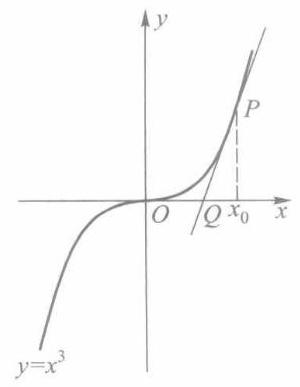
\includegraphics[width=.3\textwidth]{images/P024.jpg}
    \caption{图 $5-3$}
    \label{fig:P024}
\end{figure}

\begin{figure}
    \centering
    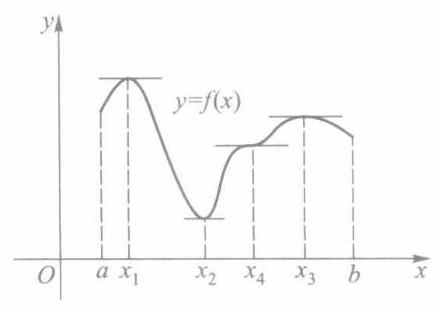
\includegraphics[width=.3\textwidth]{images/P025.jpg}
    \caption{图 $5-4$}
    \label{fig:P025}
\end{figure}

%例 8
\begin{example}
证明: 若 \({f}^{\prime }{}_{ + }\left( {x}_{0}\right)  > 0\) ,则存在 \(\delta  > 0\) ,对任何 \(x \in  \left( {{x}_{0},{x}_{0} + \delta }\right)\) ,有
\[
f\left( {x}_{0}\right)  < f\left( x\right) . \tag{10}
\]
\end{example}



%证
\begin{proof}
因为
\[
{f}_{ + }^{\prime }\left( {x}_{0}\right)  = \mathop{\lim }\limits_{{x \rightarrow  {x}_{0}^{ + }}}\frac{f\left( x\right)  - f\left( {x}_{0}\right) }{x - {x}_{0}} > 0,
\]
所以由保号性可知,存在正数 \(\delta\) ,对一切 \(x \in  \left( {{x}_{0},{x}_{0} + \delta }\right)\) ,有
\[
\frac{f\left( x\right)  - f\left( {x}_{0}\right) }{x - {x}_{0}} > 0,
\]
从而不难推得,当 \(0 < x - {x}_{0} < \delta\) 时,(10) 式成立.
\end{proof}


用类似的方法可讨论 \({f}_{ + }^{\prime }\left( {x}_{0}\right)  < 0,{f}_{ - }^{\prime }\left( {x}_{0}\right)  > 0\) 和 \({f}_{ - }^{\prime }\left( {x}_{0}\right)  < 0\) 的情况. 例如,若 \({f}_{ - }^{\prime }\left( {x}_{0}\right)  > 0\) ,则存在 \(\delta  > 0\) ,对任何 \(x \in  \left( {{x}_{0} - \delta ,{x}_{0}}\right)\) ,有 \(f\left( {x}_{0}\right)  > f\left( x\right)\) .

%注
\begin{remark}
例 8 告诉我们: 若 \({f}^{\prime }\left( {x}_{0}\right)\) 存在且不为零,则 \({x}_{0}\) 不是 \(f\left( x\right)\) 的极值点.
\end{remark}


这样我们就得到了著名的费马定理.

%定理 5.3
\begin{theorem}{费马定理}{the:费马定理}
设函数 \(f\) 在点 \({x}_{0}\) 的某邻域上有定义,且在点 \({x}_{0}\) 可导. 若点 \({x}_{0}\) 为 \(f\) 的极值点,则必有
\[
{f}^{\prime }\left( {x}_{0}\right)  = 0.
\]
\end{theorem}

费马定理的几何意义非常明确: 若函数 \(f\left( x\right)\) 在极值点 \(x = {x}_{0}\) 可导,那么在该点的切线平行于 \(x\) 轴.

我们称满足方程 \({f}^{\prime }\left( x\right)  = 0\) 的点为稳定点 (也称为驻点).

对于函数 \(f\left( x\right)  = {x}^{3}\) ,点 \(x = 0\) 是稳定点,但却不是极值点.

\subsection{习题 5.1}

1. 已知直线运动方程为
\[
s = {10t} + 5{t}^{2},
\]
分别令 \({\Delta t} = 1,{0.1},{0.01}\) ,求从 \(t = 4\) 至 \(t = 4 + {\Delta t}\) 这一段时间内运动的平均速度及 \(t = 4\) 时的瞬时速度.

2. 等速旋转的角速度等于旋转角与对应时间的比,试由此给出变速旋转的角速度的定义.

3. 设 \(f\left( {x}_{0}\right)  = 0,{f}^{\prime }\left( {x}_{0}\right)  = 4\) ,试求极限
\[
\mathop{\lim }\limits_{{{\Delta x} \rightarrow  0}}\frac{f\left( {{x}_{0} + {\Delta x}}\right) }{\Delta x}.
\]

4. 设 \(f\left( x\right)  = \left\{  \begin{matrix} {x}^{2}, & x \geq  3, \\  {ax} + b, & x < 3, \end{matrix}\right.\) 试确定 \(a,b\) 的值,使 \(f\) 在 \(x = 3\) 处可导.

5. 试确定曲线 \(y = \ln x\) 上哪些点的切线平行于下列直线:

(1) \(y = x - 1\) ;

(2) \(y = {2x} - 3\) .

6. 求下列曲线在指定点 \(P\) 的切线方程与法线方程:

(1) \(y = \frac{{x}^{2}}{4},P\left( {2,1}\right)\) ;

(2) \(y = \cos x,P\left( {0,1}\right)\) .

7. 求下列函数的导函数:

(1) \(f\left( x\right)  = {\left| x\right| }^{3}\) ;

(2) \(f\left( x\right)  = \left\{  \begin{matrix} x + 1, & x \geq  0, \\  1, & x < 0. \end{matrix}\right.\)

8. 设函数
\[
f\left( x\right)  = \left\{  {\begin{matrix} {x}^{m}\sin \frac{1}{x}, & x \neq  0, \\  0, & x = 0 \end{matrix}\left( {m\text{ 为正整数 }}\right) ,}\right.
\]
试问: (1) \(m\) 等于何值时, \(f\) 在 \(x = 0\) 连续;

(2) \(m\) 等于何值时, \(f\) 在 \(x = 0\) 可导.

9. 求下列函数的稳定点:

(1) \(f\left( x\right)  = \sin x - \cos x\) ;

(2) \(f\left( x\right)  = x - \ln x\) .

10. 设函数 \(f\) 在点 \({x}_{0}\) 存在左、右导数,试证 \(f\) 在点 \({x}_{0}\) 连续.

11. 设 \(g\left( 0\right)  = {g}^{\prime }\left( 0\right)  = 0\) ,

求 \({f}^{\prime }\left( 0\right)\) .
\[
f\left( x\right)  = \left\{  \begin{matrix} g\left( x\right) \sin \frac{1}{x}, & x \neq  0, \\  0, & x = 0, \end{matrix}\right.
\]

12. 设 \(f\) 是定义在 \(\mathbf{R}\) 上的函数,且对任何 \({x}_{1},{x}_{2} \in  \mathbf{R}\) ,都有
\[
f\left( {{x}_{1} + {x}_{2}}\right)  = f\left( {x}_{1}\right)  \cdot  f\left( {x}_{2}\right) .
\]
若 \({f}^{\prime }\left( 0\right)  = 1\) ,证明对任何 \(x \in  \mathbf{R}\) ,都有
\[
{f}^{\prime }\left( x\right)  = f\left( x\right) .
\]

13. 证明: 若 \({f}^{\prime }\left( {x}_{0}\right)\) 存在,则
\[
\mathop{\lim }\limits_{{{\Delta x} \rightarrow  0}}\frac{f\left( {{x}_{0} + {\Delta x}}\right)  - f\left( {{x}_{0} - {\Delta x}}\right) }{\Delta x} = 2{f}^{\prime }\left( {x}_{0}\right) .
\]

14. 证明: 若函数 \(f\) 在 \(\left\lbrack  {a,b}\right\rbrack\) 上连续,且 \(f\left( a\right)  = f\left( b\right)  = K,{f}_{ + }^{\prime }\left( a\right) {f}_{ - }^{\prime }\left( b\right)  > 0\) ,则至少有一点 \(\xi  \in\) (a, b),使 \(f\left( \xi \right)  = K\) .

15. 设有一吊桥,其铁链呈抛物线形,两端系于相距 \({100}\mathrm{\;m}\) 高度相同的支柱上,铁链之最低点在悬点下 \({10}\mathrm{\;m}\) 处,求铁链与支柱所成之角.

16. 在曲线 \(y = {x}^{3}\) 上取一点 \(P\) ,过 \(P\) 的切线与该曲线交于 \(Q\) ,证明: 曲线在 \(Q\) 处的切线斜率正好是在 \(P\) 处切线斜率的四倍.

17. 设 \(f\left( x\right)  = {x}^{n} + {a}_{1}{x}^{n - 1} + \cdots  + {a}_{n}\) 的最大零点为 \({x}_{0}\) . 证明: \({f}^{\prime }\left( {x}_{0}\right)  \geq  0\) .

\section{求导法则}

上一节我们从定义出发求出了一些简单函数的导数, 对于一般函数的导数, 虽然也可以用定义来求, 但通常极为繁琐. 本节将引入一些求导法则, 利用这些法则, 能较简便地求出初等函数的导数.

\subsection{导数的四则运算}

%定理 5.4
\begin{theorem}{和与差的导数}{the:和与差的导数}
若函数 \(u\left( x\right)\) 和 \(v\left( x\right)\) 在点 \({x}_{0}\) 可导,则函数 \(f\left( x\right)  = u\left( x\right)  \pm  v\left( x\right)\) 在点 \({x}_{0}\) 也可导, 且
\[
{f}^{\prime }\left( {x}_{0}\right)  = {u}^{\prime }\left( {x}_{0}\right)  \pm  {v}^{\prime }\left( {x}_{0}\right) . \tag{1}
\]
\end{theorem}

%证
\begin{proof}
\[
{f}^{\prime }\left( {x}_{0}\right)  = \mathop{\lim }\limits_{{{\Delta x} \rightarrow  0}}\frac{\left\lbrack  {u\left( {{x}_{0} + {\Delta x}}\right)  \pm  v\left( {{x}_{0} + {\Delta x}}\right) }\right\rbrack   - \left\lbrack  {u\left( {x}_{0}\right)  \pm  v\left( {x}_{0}\right) }\right\rbrack  }{\Delta x}
\]
\[
= \mathop{\lim }\limits_{{{\Delta x} \rightarrow  0}}\frac{u\left( {{x}_{0} + {\Delta x}}\right)  - u\left( {x}_{0}\right) }{\Delta x} \pm  \mathop{\lim }\limits_{{{\Delta x} \rightarrow  0}}\frac{v\left( {{x}_{0} + {\Delta x}}\right)  - v\left( {x}_{0}\right) }{\Delta x}
\]
\[
= {u}^{\prime }\left( {x}_{0}\right)  \pm  {v}^{\prime }\left( {x}_{0}\right) .
\]
\end{proof}

%定理 5.5
\begin{theorem}{积的导数}{the:积的导数}
若函数 \(u\left( x\right)\) 和 \(v\left( x\right)\) 在点 \({x}_{0}\) 可导,则函数 \(f\left( x\right)  = u\left( x\right) v\left( x\right)\) 在点 \({x}_{0}\) 也可导, 且
\[
{f}^{\prime }\left( {x}_{0}\right)  = {u}^{\prime }\left( {x}_{0}\right) v\left( {x}_{0}\right)  + u\left( {x}_{0}\right) {v}^{\prime }\left( {x}_{0}\right) . \tag{2}
\]
\end{theorem}

%证
\begin{proof}
\({f}^{\prime }\left( {x}_{0}\right)  = \mathop{\lim }\limits_{{{\Delta x} \rightarrow  0}}\frac{u\left( {{x}_{0} + {\Delta x}}\right) v\left( {{x}_{0} + {\Delta x}}\right)  - u\left( {x}_{0}\right) v\left( {x}_{0}\right) }{\Delta x}\)
\[
= \mathop{\lim }\limits_{{{\Delta x} \rightarrow  0}}\frac{u\left( {{x}_{0} + {\Delta x}}\right) v\left( {{x}_{0} + {\Delta x}}\right)  - u\left( {x}_{0}\right) v\left( {{x}_{0} + {\Delta x}}\right)  + u\left( {x}_{0}\right) v\left( {{x}_{0} + {\Delta x}}\right)  - u\left( {x}_{0}\right) v\left( {x}_{0}\right) }{\Delta x}
\]
\[
= \mathop{\lim }\limits_{{{\Delta x} \rightarrow  0}}\frac{u\left( {{x}_{0} + {\Delta x}}\right)  - u\left( {x}_{0}\right) }{\Delta x}v\left( {{x}_{0} + {\Delta x}}\right)  + \mathop{\lim }\limits_{{{\Delta x} \rightarrow  0}}u\left( {x}_{0}\right) \frac{v\left( {{x}_{0} + {\Delta x}}\right)  - v\left( {x}_{0}\right) }{\Delta x}
\]
\[
= {u}^{\prime }\left( {x}_{0}\right) v\left( {x}_{0}\right)  + u\left( {x}_{0}\right) {v}^{\prime }\left( {x}_{0}\right) .
\]
\end{proof}

利用数学归纳法可以把这个法则推广到任意有限个函数乘积的情形. 例如:
\[
{\left( uvw\right) }^{\prime } = {u}^{\prime }{vw} + u{v}^{\prime }w + {uv}{w}^{\prime }.
\]

\begin{corollary}{导数的推论}{pro:导数的推论}
若函数 \(v\left( x\right)\) 在点 \({x}_{0}\) 可导, \(c\) 为常数,则
\[
{\left( cv\left( x\right) \right) }_{x = {x}_{0}}^{\prime } = c{v}^{\prime }\left( {x}_{0}\right) . \tag{3}
\]
\end{corollary}

%例 1
\begin{example}
设 \(f\left( x\right)  = {x}^{3} + 5{x}^{2} - {9x} + \pi\) ,求 \({f}^{\prime }\left( x\right)\) .
\end{example}


%解
\begin{solution}
由公式 (1)、(3) ,
\[
{f}^{\prime }\left( x\right)  = {\left( {x}^{3}\right) }^{\prime } + 5{\left( {x}^{2}\right) }^{\prime } - 9{\left( x\right) }^{\prime } + {\left( \pi \right) }^{\prime }
\]
\[
= 3{x}^{2} + {10x} - 9\text{ . }
\]
\end{solution}

一般地说:多项式函数
\[
f\left( x\right)  = {a}_{0}{x}^{n} + {a}_{1}{x}^{n - 1} + \cdots  + {a}_{n - 1}x + {a}_{n}
\]
的导数为
\[
{f}^{\prime }\left( x\right)  = n{a}_{0}{x}^{n - 1} + \left( {n - 1}\right) {a}_{1}{x}^{n - 2} + \cdots  + {a}_{n - 1}.
\]
它比 \(f\) 低一个幂次.

%例 2
\begin{example}
设 \(y = \cos x\ln x\) ,求 \({\left. {y}^{\prime }\right| }_{x = \pi }\) .
\end{example}


%解
\begin{solution}
由公式 (2),
\[
{y}^{\prime } = {\left( \cos x\right) }^{\prime }\ln x + \cos x{\left( \ln x\right) }^{\prime } =  - \sin x\ln x + \frac{1}{x}\cos x.
\]
所以
\[
{\left. {y}^{\prime }\right| }_{x = \pi } =  - \frac{1}{\pi },
\]
\end{solution}

%定理 5.6
\begin{theorem}{商的导数}{the:}
若函数 \(u\left( x\right)\) 和 \(v\left( x\right)\) 在点 \({x}_{0}\) 都可导,且 \(v\left( {x}_{0}\right)  \neq  0\) ,则 \(f\left( x\right)  = \frac{u\left( x\right) }{v\left( x\right) }\) 在点 \({x}_{0}\) 也可导,且
\[
{f}^{\prime }\left( {x}_{0}\right)  = \frac{{u}^{\prime }\left( {x}_{0}\right) v\left( {x}_{0}\right)  - u\left( {x}_{0}\right) {v}^{\prime }\left( {x}_{0}\right) }{{\left\lbrack  v\left( {x}_{0}\right) \right\rbrack  }^{2}}. \tag{4}
\]
\end{theorem}

%证
\begin{proof}
设 \(f\left( x\right)  = u\left( x\right) g\left( x\right)\) ,其中 \(g\left( x\right)  = \frac{1}{v\left( x\right) }\) ,现证 \(g\left( x\right)\) 在点 \({x}_{0}\) 可导. 由于
\[
\frac{g\left( {{x}_{0} + {\Delta x}}\right)  - g\left( {x}_{0}\right) }{\Delta x} = \frac{\frac{1}{v\left( {{x}_{0} + {\Delta x}}\right) } - \frac{1}{v\left( {x}_{0}\right) }}{\Delta x}
\]
\[
=  - \frac{v\left( {{x}_{0} + {\Delta x}}\right)  - v\left( {x}_{0}\right) }{\Delta x} \cdot  \frac{1}{v\left( {{x}_{0} + {\Delta x}}\right) v\left( {x}_{0}\right) },
\]
而 \(v\left( x\right)\) 在点 \({x}_{0}\) 可导,从而在点 \({x}_{0}\) 连续,且 \(v\left( {x}_{0}\right)  \neq  0\) ,因此
\[
{\left( \frac{1}{v\left( x\right) }\right) }_{x = {x}_{0}}^{\prime } = {g}^{\prime }\left( {x}_{0}\right)  = \mathop{\lim }\limits_{{{\Delta x} \rightarrow  0}}\frac{g\left( {{x}_{0} + {\Delta x}}\right)  - g\left( {x}_{0}\right) }{\Delta x} =  - \frac{{v}^{\prime }\left( {x}_{0}\right) }{{\left\lbrack  v\left( {x}_{0}\right) \right\rbrack  }^{2}}. \tag{5}
\]
应用公式 (2)、(5) 便证得
\[
{f}^{\prime }\left( {x}_{0}\right)  = {\left( \frac{u\left( x\right) }{v\left( x\right) }\right) }^{\prime }{}_{x = {x}_{0}} = {u}^{\prime }\left( {x}_{0}\right) \frac{1}{v\left( {x}_{0}\right) } + u\left( {x}_{0}\right) \left( {-\frac{{v}^{\prime }\left( {x}_{0}\right) }{{\left\lbrack  v\left( {x}_{0}\right) \right\rbrack  }^{2}}}\right)
\]
\[
= \frac{{u}^{\prime }\left( {x}_{0}\right) v\left( {x}_{0}\right)  - u\left( {x}_{0}\right) {v}^{\prime }\left( {x}_{0}\right) }{{\left\lbrack  v\left( {x}_{0}\right) \right\rbrack  }^{2}}.
\]
\end{proof}

%例 3
\begin{example}
证明 \({\left( {x}^{-n}\right) }^{\prime } =  - n{x}^{-n - 1}\) ,其中 \(n\) 为正整数.
\end{example}


%证
\begin{proof}
由公式 (5) 可得
\[
{\left( {x}^{-n}\right) }^{\prime } = {\left( \frac{1}{{x}^{n}}\right) }^{\prime } =  - \frac{n{x}^{n - 1}}{{x}^{2n}} =  - n{x}^{-n - 1}.
\]
\end{proof}

%例 4
\begin{example}
证明: \({\left( \tan x\right) }^{\prime } = {\sec }^{2}x,{\left( \cot x\right) }^{\prime } =  - {\csc }^{2}x\) .

\end{example}

%证
\begin{proof}
由 \(\tan x = \frac{\sin x}{\cos x}\) 及公式 (4) 可推得
\[
{\left( \tan x\right) }^{\prime } = {\left( \frac{\sin x}{\cos x}\right) }^{\prime } = \frac{{\left( \sin x\right) }^{\prime }\cos x - \sin x{\left( \cos x\right) }^{\prime }}{{\cos }^{2}x}
\]
\[
= \frac{{\cos }^{2}x + {\sin }^{2}x}{{\cos }^{2}x} = \frac{1}{{\cos }^{2}x} = {\sec }^{2}x.
\]
同理可证 \({\left( \cot x\right) }^{\prime } =  - {\csc }^{2}x\) .
\end{proof}


%例 5
\begin{example}
证明: \({\left( \sec x\right) }^{\prime } = \sec x\tan x,{\left( \csc x\right) }^{\prime } =  - \csc x\cot x\) .
\end{example}

%证
\begin{proof}
我们仍只证第一式,第二式请读者自证. 由 \(\sec x = \frac{1}{\cos x}\) 及公式 (5) 有
\[
{\left( \sec x\right) }^{\prime } = {\left( \frac{1}{\cos x}\right) }^{\prime } =  - \frac{{\left( \cos x\right) }^{\prime }}{{\cos }^{2}x} = \frac{\sin x}{{\cos }^{2}x} = \sec x\tan x.
\]
\end{proof}

\subsection{反函数的导数}

我们已经求得对数函数与三角函数的导数, 为求得它们的反函数的导数, 下面先证明反函数求导公式.

%定理 5.7
\begin{theorem}{反函数的导数}{the:反函数的导数}
设 \(y = f\left( x\right)\) 为 \(x = \varphi \left( y\right)\) 的反函数,若 \(\varphi \left( y\right)\) 在点 \({y}_{0}\) 的某邻域上连续,严格单调且 \({\varphi }^{\prime }\left( {y}_{0}\right)  \neq  0\) ,则 \(f\left( x\right)\) 在点 \({x}_{0}\left( {{x}_{0} = \varphi \left( {y}_{0}\right) }\right)\) 可导,且
\[
{f}^{\prime }\left( {x}_{0}\right)  = \frac{1}{{\varphi }^{\prime }\left( {y}_{0}\right) }. \tag{6}
\]
\end{theorem}

%证
\begin{proof}
设 \({\Delta x} = \varphi \left( {{y}_{0} + {\Delta y}}\right)  - \varphi \left( {y}_{0}\right) ,{\Delta y} = f\left( {{x}_{0} + {\Delta x}}\right)  - f\left( {x}_{0}\right)\) . 因为 \(\varphi\) 在 \({y}_{0}\) 的某邻域上连续且严格单调,故 \(f = {\varphi }^{-1}\) 在 \({x}_{0}\) 的某邻域上连续且严格单调. 从而当且仅当 \({\Delta y} = 0\) 时 \({\Delta x} = 0\) , 并且当且仅当 \({\Delta y} \rightarrow  0\) 时 \({\Delta x} \rightarrow  0\) . 由 \({\varphi }^{\prime }\left( {y}_{0}\right)  \neq  0\) ,可得
\[
{f}^{\prime }\left( {x}_{0}\right)  = \mathop{\lim }\limits_{{{\Delta x} \rightarrow  0}}\frac{\Delta y}{\Delta x} = \mathop{\lim }\limits_{{{\Delta y} \rightarrow  0}}\frac{\Delta y}{\Delta x} = \frac{1}{\mathop{\lim }\limits_{{{\Delta y} \rightarrow  0}}\frac{\Delta x}{\Delta y}} = \frac{1}{{\varphi }^{\prime }\left( {y}_{0}\right) }.
\]
\end{proof}

%例 6
\begin{example}
证明:

(i) \({\left( {a}^{x}\right) }^{\prime } = {a}^{x}\ln a\) (其中 \(a > 0,a \neq  1\) ),特别地, \({\left( {\mathrm{e}}^{x}\right) }^{\prime } = {\mathrm{e}}^{x}\) .

(ii) \({\left( \arcsin x\right) }^{\prime } = \frac{1}{\sqrt{1 - {x}^{2}}},{\left( \arccos x\right) }^{\prime } =  - \frac{1}{\sqrt{1 - {x}^{2}}}\) .

(iii) \({\left( \arctan x\right) }^{\prime } = \frac{1}{1 + {x}^{2}},{\left( \operatorname{arccot}x\right) }^{\prime } =  - \frac{1}{1 + {x}^{2}}\) .
\end{example}


%证
\begin{proof}
(i) 由于 \(y = {a}^{x},x \in  \mathbf{R}\) 为对数函数 \(x = {\log }_{a}y,y \in  \left( {0, + \infty }\right)\) 的反函数,故由公式 (6)得到
\[
{\left( {a}^{x}\right) }^{\prime } = \frac{1}{{\left( {\log }_{a}y\right) }^{\prime }} = \frac{y}{{\log }_{a}\mathrm{e}} = {a}^{x}\ln a.
\]
(ii) 由于 \(y = \arcsin x,x \in  \left( {-1,1}\right)\) 是 \(x = \sin y,y \in  \left( {-\frac{\pi }{2},\frac{\pi }{2}}\right)\) 的反函数,故由公式 (6) 得到
\[
{\left( \arcsin x\right) }^{\prime } = \frac{1}{{\left( \sin y\right) }^{\prime }} = \frac{1}{\cos y} = \frac{1}{\sqrt{1 - {\sin }^{2}y}} = \frac{1}{\sqrt{1 - {x}^{2}}},x \in  \left( {-1,1}\right) .
\]
同理可证: \({\left( \arccos x\right) }^{\prime } =  - \frac{1}{\sqrt{1 - {x}^{2}}},x \in  \left( {-1,1}\right)\) .

(iii) 由于 \(y = \arctan x,x \in  \mathbf{R}\) 是 \(x = \tan y,y \in  \left( {-\frac{\pi }{2},\frac{\pi }{2}}\right)\) 的反函数,因此
\[
{\left( \arctan x\right) }^{\prime } = \frac{1}{{\left( \tan y\right) }^{\prime }} = \frac{1}{{\sec }^{2}y} = \frac{1}{1 + {\tan }^{2}y} = \frac{1}{1 + {x}^{2}},x \in  \left( {-\infty , + \infty }\right) .
\]
同理可证: \({\left( \operatorname{arccot}x\right) }^{\prime } =  - \frac{1}{1 + {x}^{2}},x \in  \left( {-\infty , + \infty }\right)\) .
\end{proof}


\subsection{复合函数的导数}

为了证明复合函数的求导公式, 我们先证明一个引理.

%引理
\begin{lemma}{引理}{pro:引理}
\(f\left( x\right)\) 在点 \({x}_{0}\) 可导的充要条件是: 在 \({x}_{0}\) 的某邻域 \(U\left( {x}_{0}\right)\) 上,存在一个在点 \({x}_{0}\) 连续的函数 \(H\left( x\right)\) ,使得
\[
f\left( x\right)  - f\left( {x}_{0}\right)  = H\left( x\right) \left( {x - {x}_{0}}\right) ,
\]
从而 \({f}^{\prime }\left( {x}_{0}\right)  = H\left( {x}_{0}\right)\) .
\end{lemma}


%证
\begin{proof}
设 \(f\left( x\right)\) 在点 \({x}_{0}\) 可导,令
\[
H\left( x\right)  = \left\{  \begin{array}{ll} \frac{f\left( x\right)  - f\left( {x}_{0}\right) }{x - {x}_{0}}, & x \in  {U}^{ \circ  }\left( {x}_{0}\right) , \\  {f}^{\prime }\left( {x}_{0}\right) , & x = {x}_{0}, \end{array}\right.
\]
则因
\[
\mathop{\lim }\limits_{{x \rightarrow  {x}_{0}}}H\left( x\right)  = \mathop{\lim }\limits_{{x \rightarrow  {x}_{0}}}\frac{f\left( x\right)  - f\left( {x}_{0}\right) }{x - {x}_{0}} = {f}^{\prime }\left( {x}_{0}\right)  = H\left( {x}_{0}\right) ,
\]
所以 \(H\left( x\right)\) 在点 \({x}_{0}\) 连续,且 \(f\left( x\right)  - f\left( {x}_{0}\right)  = H\left( x\right) \left( {x - {x}_{0}}\right) ,x \in  U\left( {x}_{0}\right)\) .

反之,设存在 \(H\left( x\right) ,x \in  U\left( {x}_{0}\right)\) ,它在点 \({x}_{0}\) 连续,且
\[
f\left( x\right)  - f\left( {x}_{0}\right)  = H\left( x\right) \left( {x - {x}_{0}}\right) ,x \in  U\left( {x}_{0}\right) .
\]
因存在极限
\[
\mathop{\lim }\limits_{{x \rightarrow  {x}_{0}}}\frac{f\left( x\right)  - f\left( {x}_{0}\right) }{x - {x}_{0}} = \mathop{\lim }\limits_{{x \rightarrow  {x}_{0}}}H\left( x\right)  = H\left( {x}_{0}\right) ,
\]
所以 \(f\left( x\right)\) 点 \({x}_{0}\) 可导,且 \({f}^{\prime }\left( {x}_{0}\right)  = H\left( {x}_{0}\right)\) .
\end{proof}


%注
\begin{remark}
引理说明了点 \({x}_{0}\) 是函数 \(g\left( x\right)  = \frac{f\left( x\right)  - f\left( {x}_{0}\right) }{x - {x}_{0}}\) 可去间断点的充要条件是 \(f\left( x\right)\) 在点 \({x}_{0}\) 可导. 这个结论可推广到向量函数的导数 (第二十三章).
\end{remark}


%定理 5.8
\begin{theorem}{}{the:}
设 \(u = \varphi \left( x\right)\) 在点 \({x}_{0}\) 可导, \(y = f\left( u\right)\) 在点 \({u}_{0} = \varphi \left( {x}_{0}\right)\) 可导,则复合函数 \(f \circ  \varphi\) 在点 \({x}_{0}\) 可导,且
\[
{\left( f \circ  \varphi \right) }^{\prime }\left( {x}_{0}\right)  = {f}^{\prime }\left( {u}_{0}\right) {\varphi }^{\prime }\left( {x}_{0}\right)  = {f}^{\prime }\left( {\varphi \left( {x}_{0}\right) }\right) {\varphi }^{\prime }\left( {x}_{0}\right) . \tag{7}
\]
\end{theorem}

%证
\begin{proof}
由 \(f\left( u\right)\) 在点 \({u}_{0}\) 可导,由引理必要性部分,存在一个在点 \({u}_{0}\) 连续的函数 \(F\left( u\right)\) , 使得 \({f}^{\prime }\left( {u}_{0}\right)  = F\left( {u}_{0}\right)\) ,且
\[
f\left( u\right)  - f\left( {u}_{0}\right)  = F\left( u\right) \left( {u - {u}_{0}}\right) ,u \in  U\left( {u}_{0}\right) .
\]
又由 \(u = \varphi \left( x\right)\) 在点 \({x}_{0}\) 可导,同理存在一个在点 \({x}_{0}\) 连续的函数 \(\Phi \left( x\right)\) ,使得 \({\varphi }^{\prime }\left( {x}_{0}\right)  =\)  \(\Phi \left( {x}_{0}\right)\) ,且
\[
\varphi \left( x\right)  - \varphi \left( {x}_{0}\right)  = \Phi \left( x\right) \left( {x - {x}_{0}}\right) ,x \in  U\left( {x}_{0}\right) .
\]
于是就有
\[
f\left( {\varphi \left( x\right) }\right)  - f\left( {\varphi \left( {x}_{0}\right) }\right)  = F\left( {\varphi \left( x\right) }\right) \left( {\varphi \left( x\right)  - \varphi \left( {x}_{0}\right) }\right)
\]
\[
= F\left( {\varphi \left( x\right) }\right) \Phi \left( x\right) \left( {x - {x}_{0}}\right) .
\]
因为 \(\varphi ,\Phi\) 在点 \({x}_{0}\) 连续, \(F\) 在点 \({u}_{0} = \varphi \left( {x}_{0}\right)\) 连续,因此 \(H\left( x\right)  = F\left( {\varphi \left( x\right) }\right) \Phi \left( x\right)\) 在点 \({x}_{0}\) 连续. 由引理充分性部分证得 \(f \circ  \varphi\) 在点 \({x}_{0}\) 可导,且
\[
{\left( f \circ  \varphi \right) }^{\prime }\left( {x}_{0}\right)  = H\left( {x}_{0}\right)  = F\left( {\varphi \left( {x}_{0}\right) }\right) \Phi \left( {x}_{0}\right)  = {f}^{\prime }\left( {u}_{0}\right) {\varphi }^{\prime }\left( {x}_{0}\right) .
\]
\end{proof}

%注
\begin{remark}
1 复合函数的求导公式 (7) 亦称为链式法则. 函数 \(y = f\left( u\right) ,u = \varphi \left( x\right)\) 的复合函数在点 \(x\) 的求导公式一般也写作
\[
\frac{\mathrm{d}y}{\mathrm{\;d}x} = \frac{\mathrm{d}y}{\mathrm{\;d}u} \cdot  \frac{\mathrm{d}u}{\mathrm{\;d}x}. \tag{8}
\]
对于由多个函数复合而得到的复合函数, 其导数公式可反复应用 (8) 式而得.
\end{remark}


%注
\begin{remark}
2 \({f}^{\prime }\left( {\varphi \left( x\right) }\right)  = {\left. {f}^{\prime }\left( u\right) \right| }_{u = \varphi \left( x\right) }\) 与 \({\left( f\left( \varphi \left( x\right) \right) \right) }^{\prime } = {f}^{\prime }\left( {\varphi \left( x\right) }\right) {\varphi }^{\prime }\left( x\right)\) 的含义不可混淆.
\end{remark}


%例 7
\begin{example}
设 \(y = \sin {x}^{2}\) ,求 \({y}^{\prime }\) .
\end{example}


%解
\begin{solution}
将 \(\sin {x}^{2}\) 看作 \(y = \sin u\) 与 \(u = {x}^{2}\) 的复合函数,故
\[
{\left( \sin {x}^{2}\right) }^{\prime } = \cos u \cdot  {2x} = {2x}\cos {x}^{2}.
\]
\end{solution}

%注
\begin{remark}
必须指出: \({\left( \sin {x}^{2}\right) }^{\prime } \neq  \cos {x}^{2}\) .
\end{remark}


%例 8
\begin{example}
设 \(\alpha\) 为实数,求幂函数 \(y = {x}^{\alpha }\left( {x > 0}\right)\) 的导数.
\end{example}


%解
\begin{solution}
因为 \(y = {x}^{\alpha } = {\mathrm{e}}^{\alpha \ln x}\) 可看作 \(y = {\mathrm{e}}^{u}\) 与 \(u = \alpha \ln x\) 的复合函数,故
\[
{\left( {x}^{\alpha }\right) }^{\prime } = {\left( {\mathrm{e}}^{\alpha \ln x}\right) }^{\prime } = {\mathrm{e}}^{\alpha \ln x} \cdot  \frac{\alpha }{x} = \alpha {x}^{\alpha  - 1}.
\]
\end{solution}

%例 9
\begin{example}
设 \(f\left( x\right)  = \sqrt{{x}^{2} + 1}\) ,求 \({f}^{\prime }\left( 0\right) ,{f}^{\prime }\left( 1\right)\) .
\end{example}


%解
\begin{solution}
由于
\[
{f}^{\prime }\left( x\right)  = {\left( \sqrt{{x}^{2} + 1}\right) }^{\prime } = \frac{1}{2\sqrt{{x}^{2} + 1}}{\left( {x}^{2} + 1\right) }^{\prime } = \frac{x}{\sqrt{{x}^{2} + 1}},
\]
因此 \({f}^{\prime }\left( 0\right)  = 0,{f}^{\prime }\left( 1\right)  = \frac{1}{\sqrt{2}}\) .
\end{solution}


%例 10
\begin{example}
求下列函数的导函数:

(1) \(f\left( x\right)  = \ln \left( {x + \sqrt{1 + {x}^{2}}}\right)\) ;

(2) \(f\left( x\right)  = {\tan }^{2}\frac{1}{x}\) .
\end{example}


%解
\begin{solution}
(1) \({\left( \ln \left( x + \sqrt{1 + {x}^{2}}\right) \right) }^{\prime } = \frac{1}{x + \sqrt{1 + {x}^{2}}}{\left( x + \sqrt{1 + {x}^{2}}\right) }^{\prime }\)
\[
= \frac{1}{x + \sqrt{1 + {x}^{2}}}\left( {1 + \frac{x}{\sqrt{1 + {x}^{2}}}}\right)  = \frac{1}{\sqrt{1 + {x}^{2}}}.
\]
(2) \({\left( {\tan }^{2}\frac{1}{x}\right) }^{\prime } = 2\tan \frac{1}{x}{\left( \tan \frac{1}{x}\right) }^{\prime } = 2\tan \frac{1}{x}{\sec }^{2}\frac{1}{x}{\left( \frac{1}{x}\right) }^{\prime }\)
\[
=  - \frac{2}{{x}^{2}}\tan \frac{1}{x}{\sec }^{2}\frac{1}{x}\text{ . }
\]
\end{solution}

%例 11
\begin{example}
(对数求导法) 设 \(y = \frac{{\left( x + 5\right) }^{2}{\left( x - 4\right) }^{\frac{1}{3}}}{{\left( x + 2\right) }^{5}{\left( x + 4\right) }^{\frac{1}{2}}}\left( {x > 4}\right)\) ,求 \({y}^{\prime }\) .
\end{example}


%解
\begin{solution}
先对函数式取对数, 得
\[
\ln y = \ln \frac{{\left( x + 5\right) }^{2}{\left( x - 4\right) }^{\frac{1}{3}}}{{\left( x + 2\right) }^{5}{\left( x + 4\right) }^{\frac{1}{2}}}
\]
\[
= 2\ln \left( {x + 5}\right)  + \frac{1}{3}\ln \left( {x - 4}\right)  - 5\ln \left( {x + 2}\right)  - \frac{1}{2}\ln \left( {x + 4}\right) .
\]
再对上式两边分别求导数, 得
\[
\frac{{y}^{\prime }}{y} = \frac{2}{x + 5} + \frac{1}{3\left( {x - 4}\right) } - \frac{5}{x + 2} - \frac{1}{2\left( {x + 4}\right) }.
\]
整理后得到
\[
{y}^{\prime } = \frac{{\left( x + 5\right) }^{2}{\left( x - 4\right) }^{\frac{1}{3}}}{{\left( x + 2\right) }^{5}{\left( x + 4\right) }^{\frac{1}{2}}}\left\lbrack  {\frac{2}{x + 5} + \frac{1}{3\left( {x - 4}\right) } - \frac{5}{x + 2} - \frac{1}{2\left( {x + 4}\right) }}\right\rbrack  .
\]
\end{solution}

%注
\begin{remark}
虽然我们可用导数的乘积和商的公式来求例 11 中的导数, 但用对数求导法显得更为清晰、简便.
\end{remark}


%例 12
\begin{example}
设 \(y = u{\left( x\right) }^{v\left( x\right) }\) ,其中 \(u\left( x\right)  > 0\) ,且 \(u\left( x\right)\) 和 \(v\left( x\right)\) 均可导,试求此幂指函数的导数.
\end{example}


%解
\begin{solution}
\[
{y}^{\prime } = {\left( u{\left( x\right) }^{v\left( x\right) }\right) }^{\prime } = {\left( {\mathrm{e}}^{v\left( x\right) \ln u\left( x\right) }\right) }^{\prime } = {\mathrm{e}}^{v\left( x\right) \ln u\left( x\right) }{\left( v\left( x\right) \ln u\left( x\right) \right) }^{\prime }
\]
\[
= u{\left( x\right) }^{v\left( x\right) }\left( {{v}^{\prime }\left( x\right) \ln u\left( x\right)  + v\left( x\right) \frac{{u}^{\prime }\left( x\right) }{u\left( x\right) }}\right)
\]
\[
= u{\left( x\right) }^{v\left( x\right) }{v}^{\prime }\left( x\right) \ln u\left( x\right)  + u{\left( x\right) }^{v\left( x\right)  - 1}{u}^{\prime }\left( x\right) v\left( x\right) .
\]
\end{solution}

\subsection{基本求导法则与公式}

现在把前面得到的求导法则与基本初等函数的导数公式列出如下:

基本求导法则

1. \({\left( u \pm  v\right) }^{\prime } = {u}^{\prime } \pm  {v}^{\prime }\) .

2. \({\left( uv\right) }^{\prime } = {u}^{\prime }v + u{v}^{\prime },{\left( cu\right) }^{\prime } = c{u}^{\prime }\;\left( {c\text{ 为常数 }}\right)\) .

3. \({\left( \frac{u}{v}\right) }^{\prime } = \frac{{u}^{\prime }v - u{v}^{\prime }}{{v}^{2}},{\left( \frac{1}{v}\right) }^{\prime } =  - \frac{{v}^{\prime }}{{v}^{2}}\;\left( {v \neq  0}\right)\) .

4. 反函数导数 \(\frac{\mathrm{d}y}{\mathrm{\;d}x} = \frac{1}{\frac{\mathrm{d}x}{\mathrm{\;d}y}}\) .

5. 复合函数导数 \(\frac{\mathrm{d}y}{\mathrm{\;d}x} = \frac{\mathrm{d}y}{\mathrm{\;d}u} \cdot  \frac{\mathrm{d}u}{\mathrm{\;d}x}\) .

基本初等函数导数公式

1. \({\left( c\right) }^{\prime } = 0\;\left( {c\text{ 为常数 }}\right)\) .

2. \({\left( {x}^{\alpha }\right) }^{\prime } = \alpha {x}^{\alpha  - 1}\;\left( {\alpha \text{ 为任意实数 }}\right)\) .

3. \({\left( \sin x\right) }^{\prime } = \cos x,{\left( \cos x\right) }^{\prime } =  - \sin x,{\left( \tan x\right) }^{\prime } = {\sec }^{2}x\) ,

\({\left( \cot x\right) }^{\prime } =  - {\csc }^{2}x,{\left( \sec x\right) }^{\prime } = \sec x\tan x,{\left( \csc x\right) }^{\prime } =  - \csc x\cot x.\)

4. \({\left( \arcsin x\right) }^{\prime } = \frac{1}{\sqrt{1 - {x}^{2}}},{\left( \arccos x\right) }^{\prime } =  - \frac{1}{\sqrt{1 - {x}^{2}}}\) ,

\({\left( \arctan x\right) }^{\prime } = \frac{1}{1 + {x}^{2}},{\left( \operatorname{arccot}x\right) }^{\prime } =  - \frac{1}{1 + {x}^{2}}.\)

5. \({\left( {a}^{x}\right) }^{\prime } = {a}^{x}\ln a\left( {a > 0\text{ 且 }a \neq  1}\right) ,{\left( {\mathrm{e}}^{x}\right) }^{\prime } = {\mathrm{e}}^{x}\) .

6. \({\left( {\log }_{a}\left| x\right| \right) }^{\prime } = \frac{1}{x\ln a}\left( {a > 0\text{ 且 }a \neq  1}\right) ,{\left( \ln \left| x\right| \right) }^{\prime } = \frac{1}{x}\) .

\subsection{习题 5.2}

1. 求下列函数在指定点的导数:

(1)设 \(f\left( x\right)  = 3{x}^{4} + 2{x}^{3} + 5\) ,求 \({f}^{\prime }\left( 0\right) ,{f}^{\prime }\left( 1\right)\) ；

(2)设 \(f\left( x\right)  = \frac{x}{\cos x}\) ,求 \({f}^{\prime }\left( 0\right) ,{f}^{\prime }\left( \pi \right)\) ；

(3)设 \(f\left( x\right)  = \sqrt{1 + \sqrt{x}}\) ,求 \({f}^{\prime }\left( 0\right)\) , \({f}^{\prime }\left( 1\right)\) , \({f}^{\prime }\left( 4\right)\) .

2. 求下列函数的导数:

(1) \(y = 3{x}^{2} + 2\) ;

(2) \(y = \frac{1 - {x}^{2}}{1 + x + {x}^{2}}\) ;

(3) \(y = {x}^{n} + {nx}\) ;

(4) \(y = \frac{x}{m} + \frac{m}{x} + 2\sqrt{x} + \frac{2}{\sqrt{x}}\) ;

(5) \(y = {x}^{3}{\log }_{3}x\) ;

(6) \(y = {\mathrm{e}}^{x}\cos x\) ;

(7) \(y = \left( {{x}^{2} + 1}\right) \left( {{3x} - 1}\right) \left( {1 - {x}^{3}}\right)\) ;

(8) \(y = \frac{\tan x}{x}\) ;

(9) \(y = \frac{x}{1 - \cos x}\) ;

(10) \(y = \frac{1 + \ln x}{1 - \ln x}\) ;

(11) \(y = \left( {\sqrt{x} + 1}\right) \arctan x\) ;

(12) \(y = \frac{1 + {x}^{2}}{\sin x + \cos x}\) .

3. 求下列函数的导函数:

(1) \(y = x\sqrt{1 - {x}^{2}}\) ;

(2) \(y = {\left( {x}^{2} - 1\right) }^{3}\) ;

(3) \(y = {\left( \frac{1 + {x}^{2}}{1 - x}\right) }^{3}\) ;

(4) \(y = \ln \left( {\ln x}\right)\) ;

(5) \(y = \ln \left( {\sin x}\right)\) ;

(6) \(y = \lg \left( {{x}^{2} + x + 1}\right)\) ;

(7) \(y = \ln \left( {x + \sqrt{1 + {x}^{2}}}\right)\) ;

(8) \(y = \ln \frac{\sqrt{1 + x} - \sqrt{1 - x}}{\sqrt{1 + x} + \sqrt{1 - x}}\) ;

(9) \(y = {\left( \sin x + \cos x\right) }^{3}\) ；

(10) \(y = {\cos }^{3}{4x}\) ;

(11) \(y = \sin \sqrt{1 + {x}^{2}}\) ;

(12) \(y = {\left( \sin {x}^{2}\right) }^{3}\) ;

(13) \(y = \arcsin \frac{1}{x}\) ;

(14) \(y = {\left( \arctan {x}^{3}\right) }^{2}\) ;

(15) \(y = \operatorname{arccot}\frac{1 + x}{1 - x}\) ;

(16) \(y = \arcsin \left( {{\sin }^{2}x}\right)\) ;

(17) \(y = {\mathrm{e}}^{x + 1}\) ;

(18) \(y = {2}^{\sin x}\) ;

(19) \(y = {x}^{\sin x}\) ;

(20) \(y = {x}^{{x}^{x}}\) ;

(21) \(y = {\mathrm{e}}^{-x}\sin {2x}\) ;

(22) \(y = \sqrt{x + \sqrt{x + \sqrt{x}}}\) ;

(23) \(y = \sin \left( {\sin \left( {\sin x}\right) }\right)\) ;

(24) \(y = \sin \left( \frac{x}{\sin \left( \frac{x}{\sin x}\right) }\right)\) ;

( 25 ) \(y = {\left( x - {a}_{1}\right) }^{{\alpha }_{1}}{\left( x - {a}_{2}\right) }^{{\alpha }_{2}}\cdots {\left( x - {a}_{n}\right) }^{{\alpha }_{n}}\) ;

( 26 ) \(y = \frac{1}{\sqrt{{a}^{2} - {b}^{2}}}\arcsin \frac{a\sin x + b}{a + b\sin x}\) .

4. 对下列各函数计算 \({f}^{\prime }\left( x\right) ,{f}^{\prime }\left( {x + 1}\right) ,{f}^{\prime }\left( {x - 1}\right)\) .

(1) \(f\left( x\right)  = {x}^{3}\) ;

(2) \(f\left( {x + 1}\right)  = {x}^{3}\) ;

(3) \(f\left( {x - 1}\right)  = {x}^{3}\) .

5. 已知 \(g\) 为可导函数, \(a\) 为实数,试求下列函数 \(f\) 的导数:

(1) \(f\left( x\right)  = g\left( {x + g\left( a\right) }\right)\) ;

(2) \(f\left( x\right)  = g\left( {x + g\left( x\right) }\right)\) ;

(3) \(f\left( x\right)  = g\left( {{xg}\left( a\right) }\right)\) ;

(4) \(f\left( x\right)  = g\left( {{xg}\left( x\right) }\right)\) .

6. 设 \(f\) 为可导函数,证明: 若 \(x = 1\) 时有
\[
\frac{\mathrm{d}}{\mathrm{d}x}f\left( {x}^{2}\right)  = \frac{\mathrm{d}}{\mathrm{d}x}{f}^{2}\left( x\right) .
\]
则必有 \({f}^{\prime }\left( 1\right)  = 0\) 或 \(f\left( 1\right)  = 1\) .

7. 定义双曲函数如下:

双曲正弦函数 \(\sinh x = \frac{{\mathrm{e}}^{x} - {\mathrm{e}}^{-x}}{2}\) ,双曲余弦函数 \(\cosh x = \frac{{\mathrm{e}}^{x} + {\mathrm{e}}^{-x}}{2}\) ;

双曲正切函数 \(\tanh x = \frac{\sin \mathrm{h}x}{\cos \mathrm{h}x}\) ,双曲余切函数 \(\coth x = \frac{\cos \mathrm{h}x}{\sin \mathrm{h}x}\) .

证明:

(1) \({\left( \sinh x\right) }^{\prime } = \cos \mathrm{h}x\) ;

(2) \({\left( \cosh x\right) }^{\prime } = \sin \mathrm{h}x\) ;

(3) \({\left( \tanh x\right) }^{\prime } = \frac{1}{\cos {\mathrm{h}}^{2}x}\) ;

(4) \({\left( \coth x\right) }^{\prime } =  - \frac{1}{\sin {\mathrm{h}}^{2}x}\) .

8. 求下列函数的导数:

(1) \(y = {\sinh }^{3}x\) ;

(2) \(y = \cosh \left( {\sinh x}\right)\) ;

(3) \(y = \ln \left( {\cosh x}\right)\) ;

(4) \(y = \arctan \left( {\tanh x}\right)\) .

9. 以 arsinh \(x\) , arcosh \(x\) , artanh \(x\) , arcoth \(x\) 分别表示各双曲函数的反函数. 试求下列函数的导数:

(1) \(y = \operatorname{arsinh}x\) ;

(2) \(y = \operatorname{arcosh}x\) ;

(3) \(y = \operatorname{artanh}x\) ;

(4) \(y = \operatorname{arcoth}x\) ;

(5) \(y = \operatorname{artanh}x - \operatorname{arcoth}\frac{1}{x}\) ;

(6) \(y = \operatorname{arsinh}\left( {\tan x}\right)\) .

\section{参变量函数的导数}

平面曲线 \(C\) 一般的表达形式是参变量 (参量) 方程
\[
\left\{  {\begin{array}{l} x = \varphi \left( t\right) , \\  y = \psi \left( t\right) , \end{array}\;\alpha  \leq  t \leq  \beta }\right.
\]
(1) 表示. 设 \(t = {t}_{0}\) 对应曲线 \(C\) 上的点 \(P\) . 如果在点 \(P\) 有切线,那么切线的斜率可由割线的斜率取极限而得,为此设 \(\varphi ,\psi\) 在点 \({t}_{0}\) 可导,且 \({x}^{\prime }\left( {t}_{0}\right)  \neq  0\) . 若 \({t}_{0} + {\Delta t}\) 对应 \(C\) 上的点 \(Q\) (图5-5),割线 \({PQ}\) 的斜率
\[
\frac{\Delta y}{\Delta x} = \frac{\psi \left( {{t}_{0} + {\Delta t}}\right)  - \psi \left( {t}_{0}\right) }{\varphi \left( {{t}_{0} + {\Delta t}}\right)  - \varphi \left( {t}_{0}\right) },
\]
\begin{figure}
	\centering
	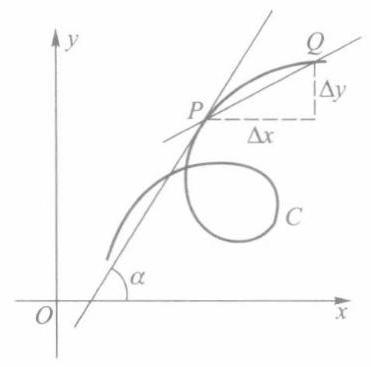
\includegraphics[width=.3\textwidth]{images/P026.jpg}
	\caption{图 $5-5$}
	\label{fig:P026}
\end{figure}

于是曲线 \(C\) 在点 \(P\) 的切线斜率是
\[
\tan \alpha  = \mathop{\lim }\limits_{{{\Delta t} \rightarrow  0}}\frac{\Delta y}{\Delta x} = \frac{\mathop{\lim }\limits_{{{\Delta t} \rightarrow  0}}\frac{\psi \left( {{t}_{0} + {\Delta t}}\right)  - \psi \left( {t}_{0}\right) }{\Delta t}}{\mathop{\lim }\limits_{{{\Delta t} \rightarrow  0}}\frac{\varphi \left( {{t}_{0} + {\Delta t}}\right)  - \varphi \left( {t}_{0}\right) }{\Delta t}}
= \frac{{\psi }^{\prime }\left( {t}_{0}\right) }{{\varphi }^{\prime }\left( {t}_{0}\right) }.
\]
其中 \(\alpha\) 为切线与 \(x\) 轴正向的夹角. 若 \({\varphi }^{\prime }\left( {t}_{0}\right)  = 0\) ,但 \({\psi }^{\prime }\left( {t}_{0}\right)  \neq  0\) ,同样可得
\[
\cot \alpha  = \mathop{\lim }\limits_{{{\Delta t} \rightarrow  0}}\frac{\Delta x}{\Delta y} = \frac{{\varphi }^{\prime }\left( {t}_{0}\right) }{{\psi }^{\prime }\left( {t}_{0}\right) }.
\]
若 \(\varphi ,\psi\) 在 \(\left\lbrack  {\alpha ,\beta }\right\rbrack\) 上都存在连续的导函数,且 \({\varphi }^{\prime 2} + {\psi }^{\prime 2} \neq  0\) ,这时称 \(C\) 为光滑曲线. 其特点是在曲线 \(C\) 上不仅每一点都有切线,且切线与 \(x\) 轴正向的夹角 \(\alpha \left( t\right)\) 是 \(t\) 的连续函数.

若 \(x = \varphi \left( t\right)\) 具有反函数 \(t = {\varphi }^{-1}\left( x\right)\) ,那么它与 \(y = \psi \left( t\right)\) 构成一个复合函数
\[
y = \psi  \circ  {\varphi }^{-1}\left( x\right) .
\]
这时只要函数 \(\varphi ,\psi\) 可导, \({\varphi }^{\prime }\left( t\right)  \neq  0\) (因而当 \({\Delta x} \rightarrow  0\) 时,也有 \({\Delta t} \rightarrow  0\) 和 \({\Delta y} \rightarrow  0\) ),就可由复合函数和反函数的求导法则得到
\[
\frac{\mathrm{d}y}{\mathrm{\;d}x} = \frac{\mathrm{d}y}{\mathrm{\;d}t} \cdot  \frac{\mathrm{d}t}{\mathrm{\;d}x} = \frac{\mathrm{d}y}{\mathrm{\;d}t}/\frac{\mathrm{d}x}{\mathrm{\;d}t} = \frac{{\psi }^{\prime }\left( t\right) }{{\varphi }^{\prime }\left( t\right) }. \tag{2}
\]
%例 1
\begin{example}
试求由上半椭圆的参量方程
\[
\left\{  {\begin{array}{l} x = a\cos t, \\  y = b\sin t, \end{array}\;0 < t < \pi }\right.
\]
所确定的函数 \(y = y\left( x\right)\) 的导数.
\end{example}


%解
\begin{solution}
按公式(2)求得
\[
\frac{\mathrm{d}y}{\mathrm{\;d}x} = \frac{\mathrm{d}y}{\mathrm{\;d}t}/\frac{\mathrm{d}x}{\mathrm{\;d}t} = \frac{{\left( b\sin t\right) }^{\prime }}{{\left( a\cos t\right) }^{\prime }} =  - \frac{b}{a}\cot t.
\]
若曲线 \(C\) 由极坐标 \(r = r\left( \theta \right)\) 表示,则可转化为以极角 \(\theta\) 为参量的参量方程:
\[
\left\{  \begin{array}{l} x = r\cos \theta  = r\left( \theta \right) \cos \theta , \\  y = r\sin \theta  = r\left( \theta \right) \sin \theta . \end{array}\right.
\]
这时在相应的条件下可得
\[
\frac{\mathrm{d}y}{\mathrm{\;d}x} = \frac{{\left( r\left( \theta \right) \sin \theta \right) }^{\prime }}{{\left( r\left( \theta \right) \cos \theta \right) }^{\prime }} = \frac{{r}^{\prime }\left( \theta \right) \sin \theta  + r\left( \theta \right) \cos \theta }{{r}^{\prime }\left( \theta \right) \cos \theta  - r\left( \theta \right) \sin \theta } = \frac{{r}^{\prime }\left( \theta \right) \tan \theta  + r\left( \theta \right) }{{r}^{\prime }\left( \theta \right)  - r\left( \theta \right) \tan \theta }. \tag{3}
\]
(3) 式表示在曲线 \(r = r\left( \theta \right)\) 上的点 \(M\left( {r,\theta }\right)\) 的切线 \({MT}\) 与极轴 \({Ox}\) 轴的夹角的正切 (图 5-6).

过点 \(M\) 的射线 \({OH}\) 与切线 \({MT}\) 的夹角 \(\varphi\) 的正切则是
\[
\tan \varphi  = \tan \left( {\alpha  - \theta }\right)  = \frac{\tan \alpha  - \tan \theta }{1 + \tan \alpha \tan \theta }. \tag{4}
\]
将 (3) 式代入 (4) 式则得向径与切线夹角的正切
\[
\tan \varphi  = \frac{r\left( \theta \right) }{{r}^{\prime }\left( \theta \right) }. \tag{5}
\]
\end{solution}

%例 2
\begin{example}
证明: 对数螺线 \(r = {\mathrm{e}}^{\frac{\theta }{2}}\) (图 5-7) 上所有点的切线与向径的夹角 \(\varphi\) 为常量.
\end{example}


%证
\begin{proof}
由 (5) 式得,对每一 \(\theta\) 值都有
\[
\tan \varphi  = \frac{r\left( \theta \right) }{{r}^{\prime }\left( \theta \right) } = \frac{{\mathrm{e}}^{\frac{\theta }{2}}}{\frac{1}{2}{\mathrm{e}}^{\frac{\theta }{2}}} = 2,
\]
\begin{figure}
    \centering
    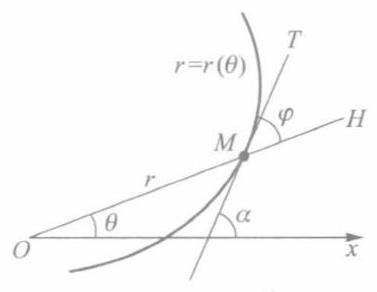
\includegraphics[width=.3\textwidth]{images/P027.jpg}
    \caption{图 $5-6$}
    \label{fig:P027}
\end{figure}

\begin{figure}
    \centering
    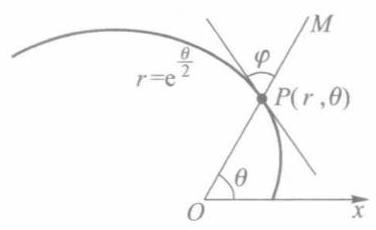
\includegraphics[width=.3\textwidth]{images/P028.jpg}
    \caption{图 $5-7$}
    \label{fig:P028}
\end{figure}

即在对数螺线上任一点的切线与向径的夹角等于 \(\arctan 2\) .
\end{proof}


\subsection{习题 5.3}

1. 求下列由参量方程所确定的导数 \(\frac{\mathrm{d}y}{\mathrm{\;d}x}\) :

(1) \(\left\{  \begin{array}{l} x = {\cos }^{4}t, \\  y = {\sin }^{4}t \end{array}\right.\) 在 \(t = \frac{\pi }{3}\) 处; (2) \(\left\{  \begin{array}{l} x = \frac{t}{1 + t}, \\  y = \frac{1 - t}{1 + t} \end{array}\right.\) 在 \(t > 0\) 处.

2. 设 \(\left\{  {\begin{array}{l} x = a\left( {t - \sin t}\right) , \\  y = a\left( {1 - \cos t}\right) . \end{array}\text{ 求 }{\left. \frac{\mathrm{d}y}{\mathrm{\;d}x}\right| }_{t = \frac{\pi }{2}}}\right.\) , \({\left. \frac{\mathrm{d}y}{\mathrm{\;d}x}\right| }_{t = \pi }\) .

3. 设曲线方程 \(x = 1 - {t}^{2},y = t - {t}^{2}\) ,求它在下列点处的切线方程与法线方程:

(1) \(t = 1\) ;

(2) \(t = \frac{\sqrt{2}}{2}\) .

4. 证明曲线
\[
\left\{  \begin{array}{l} x = a\left( {\cos t + t\sin t}\right) , \\  y = a\left( {\sin t - t\cos t}\right)  \end{array}\right.
\]
上任一点的法线到原点距离等于 \(a\) .

5. 证明: 圆 \(r = {2a}\sin \theta \left( {a > 0}\right)\) 上任一点的切线与向径的夹角等于向径的极角.

6. 求心形线 \(r = a\left( {1 + \cos \theta }\right)\) 的切线与切点向径之间的夹角.

\section{高阶导数}

设物体的运动方程为 \(s = s\left( t\right)\) ,则物体的运动速度为 \(v\left( t\right)  = {s}^{\prime }\left( t\right)\) ,而速度在时刻 \({t}_{0}\) 的变化率
\[
\mathop{\lim }\limits_{{{\Delta t} \rightarrow  0}}\frac{v\left( {{t}_{0} + {\Delta t}}\right)  - v\left( {t}_{0}\right) }{\Delta t} = \mathop{\lim }\limits_{{t \rightarrow  {t}_{0}}}\frac{v\left( t\right)  - v\left( {t}_{0}\right) }{t - {t}_{0}}
\]
就是运动物体在时刻 \({t}_{0}\) 的加速度. 因此,加速度是速度函数的导数,也就是路程 \(s\left( t\right)\) 的导函数的导数, 这就产生了高阶导数的概念.

%定义  1
\begin{definition}{二阶导数}{def:二阶导数}
若函数 \(f\) 的导函数 \({f}^{\prime }\) 在点 \({x}_{0}\) 可导,则称 \({f}^{\prime }\) 在点 \({x}_{0}\) 的导数为 \(f\) 在点 \({x}_{0}\) 的二阶导数,记作 \({f}^{\prime \prime }\left( {x}_{0}\right)\) ,即
\[
\mathop{\lim }\limits_{{x \rightarrow  {x}_{0}}}\frac{{f}^{\prime }\left( x\right)  - {f}^{\prime }\left( {x}_{0}\right) }{x - {x}_{0}} = {f}^{\prime \prime }\left( {x}_{0}\right) ,
\]
同时称 \(f\) 在点 \({x}_{0}\) 为二阶可导.
\end{definition}


若 \(f\) 在区间 \(I\) 上每一点都二阶可导,则得到一个定义在 \(I\) 上的函数,这个函数称为 \(f\) 的二阶导函数,记作 \({f}^{\prime \prime }\left( x\right) ,x \in  I\) ,或者简单记为 \({f}^{\prime \prime }\) .

一般地,可由 \(f\) 的 \(n - 1\) 阶导函数定义 \(f\) 的 \(n\) 阶导函数 (或简称 \(n\) 阶导数).

二阶以及二阶以上的导数都称为高阶导数,函数 \(f\) 在点 \({x}_{0}\) 处的 \(n\) 阶导数记作
\[
{f}^{\left( n\right) }\left( {x}_{0}\right) ,{\left. {y}^{\left( n\right) }\right| }_{x = {x}_{0}}\text{ 或 }{\left. \frac{{\mathrm{d}}^{n}y}{\mathrm{\;d}{x}^{n}}\right| }_{x = {x}_{0}}\text{ . }
\]
相应地, \(n\) 阶导函数记作
\[
{f}^{\left( n\right) },{y}^{\left( n\right) }\text{ 或 }\frac{{\mathrm{d}}^{n}y}{\mathrm{\;d}{x}^{n}}\text{ . }
\]
这里 \(\frac{{\mathrm{d}}^{n}y}{\mathrm{\;d}{x}^{n}}\) 亦可写作 \(\frac{{\mathrm{d}}^{n}}{\mathrm{\;d}{x}^{n}}y\) ,它是对 \(y\) 相继进行 \(n\) 次求导运算 “ \(\frac{\mathrm{d}}{\mathrm{d}x}\) ” 的结果.

%例 1
\begin{example}
求幂函数 \(y = {x}^{n}\) ( \(n\) 为正整数) 的各阶导数.
\end{example}


%解
\begin{solution}
由幂函数的求导公式得
\[
{y}^{\prime } = n{x}^{n - 1},
\]
\[
{y}^{\prime \prime } = n\left( {n - 1}\right) {x}^{n - 2},
\]
............
\[
{y}^{\left( n - 1\right) } = {\left( {y}^{\left( n - 2\right) }\right) }^{\prime } = n\left( {n - 1}\right) \cdots {2x},
\]
\[
{y}^{\left( n\right) } = {\left( {y}^{\left( n - 1\right) }\right) }^{\prime } = {\left( n\left( n - 1\right) \cdots 2x\right) }^{\prime } = n!,
\]
\[
{y}^{\left( n + 1\right) } = {y}^{\left( n + 2\right) } = \cdots  = 0.
\]
由此可见,对于正整数幂函数 \({x}^{n}\) ,每求导一次,其幂次降低 1,第 \(n\) 阶导数为一常数,大于 \(n\) 阶的导数都等于 0 .
\end{solution}


%例 2
\begin{example}
求 \(y = \sin x\) 和 \(y = \cos x\) 的各阶导数.
\end{example}


%解
\begin{solution}
对于 \(y = \sin x\) ,由三角函数的求导公式得
\[
{y}^{\prime } = \cos x,{y}^{\prime \prime } =  - \sin x,{y}^{\prime \prime \prime } =  - \cos x,{y}^{\left( 4\right) } = \sin x.
\]
继续求导,将出现周而复始的现象. 为了得到一般 \(n\) 阶导数公式,可将上述导数公式改写为
\[
{y}^{\prime } = \cos x = \sin \left( {x + \frac{\pi }{2}}\right) ,
\]
\[
{y}^{\prime \prime } =  - \sin x = \sin \left( {x + 2 \cdot  \frac{\pi }{2}}\right) ,
\]
\[
{y}^{\prime \prime \prime } =  - \cos x = \sin \left( {x + 3 \cdot  \frac{\pi }{2}}\right) ,
\]
\[
{y}^{\left( 4\right) } = \sin x = \sin \left( {x + 4 \cdot  \frac{\pi }{2}}\right) .
\]
一般地, 可推得
\[
{y}^{\left( n\right) } = \sin \left( {x + n \cdot  \frac{\pi }{2}}\right) ,n \in  {\mathbf{N}}_{ + }.
\]
类似地有
\[
{\cos }^{\left( n\right) }x = \cos \left( {x + n \cdot  \frac{\pi }{2}}\right) ,n \in  {\mathbf{N}}_{ + }.
\]
\end{solution}

%例 3
\begin{example}
求 \(y = {\mathrm{e}}^{x}\) 的各阶导数.
\end{example}


%解
\begin{solution}
因为 \({\left( {\mathrm{e}}^{x}\right) }^{\prime } = {\mathrm{e}}^{x}\) ,所以 \({\left( {\mathrm{e}}^{x}\right) }^{\left( n\right) } = {\mathrm{e}}^{x},n \in  {\mathbf{N}}_{ + }\) .
\end{solution}


指数函数 \({\mathrm{e}}^{x}\) 的各阶导数仍旧是 \({\mathrm{e}}^{x}\) .

一阶导数的运算法则可直接移植到高阶导数. 容易看出:
\[
{\left\lbrack  u \pm  v\right\rbrack  }^{\left( n\right) } = {u}^{\left( n\right) } \pm  {v}^{\left( n\right) }. \tag{1}
\]
对于乘法求导法则较为复杂一些. 设 \(y = {uv}\) ,则
\[
{y}^{\prime } = {u}^{\prime }v + u{v}^{\prime },
\]
\[
{y}^{\prime \prime } = {\left( {u}^{\prime }v + u{v}^{\prime }\right) }^{\prime } = {u}^{\prime \prime }v + 2{u}^{\prime }{v}^{\prime } + u{v}^{\prime \prime },
\]
\[
{y}^{\prime \prime \prime } = {\left( {u}^{\prime \prime }v + 2{u}^{\prime }{v}^{\prime } + u{v}^{\prime \prime }\right) }^{\prime } = {u}^{\prime \prime \prime }v + 3{u}^{\prime \prime }{v}^{\prime } + 3{u}^{\prime }{v}^{\prime \prime } + u{v}^{\prime \prime \prime },
\]
如此下去,读者不难看到,计算结果与二项式 \({\left( u + v\right) }^{n}\) 展开式极为相似,用数学归纳法, 可得
\[
{\left( uv\right) }^{\left( n\right) } = {u}^{\left( n\right) }{v}^{\left( 0\right) } + {\mathrm{C}}_{n}^{1}{u}^{\left( n - 1\right) }{v}^{\left( 1\right) } + {\mathrm{C}}_{n}^{2}{u}^{\left( n - 2\right) }{v}^{\left( 2\right) } + \cdots  +
\]
\[
{\mathrm{C}}_{n}^{k}{u}^{\left( n - k\right) }{v}^{\left( k\right) } + \cdots  + {u}^{\left( 0\right) }{v}^{\left( n\right) } = \mathop{\sum }\limits_{{k = 0}}^{n}{\mathrm{C}}_{n}^{k}{u}^{\left( n - k\right) }{v}^{\left( k\right) }, \tag{2}
\]
其中 \({u}^{\left( 0\right) } = u,{v}^{\left( 0\right) } = v\) . 这个公式称为莱布尼茨公式.

%例 4
\begin{example}
设 \(y = {x}^{2}{\mathrm{e}}^{x}\) ,求 \({y}^{\left( n\right) }\) .
\end{example}


%解
\begin{solution}
令 \(u\left( x\right)  = {\mathrm{e}}^{x},v\left( x\right)  = {x}^{2}\) ,应用莱布尼茨公式得
\[
{y}^{\left( n\right) } = \mathop{\sum }\limits_{{k = 0}}^{n}{\mathrm{C}}_{n}^{k}{u}^{\left( n - k\right) }{v}^{\left( k\right) } = \mathop{\sum }\limits_{{k = 0}}^{n}{\mathrm{C}}_{n}^{k}{v}^{\left( k\right) }{\mathrm{e}}^{x}
\]
\[
= {x}^{2}{\mathrm{e}}^{x} + {2nx}{\mathrm{e}}^{x} + n\left( {n - 1}\right) {\mathrm{e}}^{x} = {\mathrm{e}}^{x}\left\lbrack  {{x}^{2} + {2nx} + n\left( {n - 1}\right) }\right\rbrack  .
\]
\end{solution}

%例 5
\begin{example}
设 \(y = {\mathrm{e}}^{x}\sin x\) ,求 \({y}^{\left( n\right) }\) .
\end{example}


%解
\begin{solution}
因为
\[
{y}^{\prime } = {\mathrm{e}}^{x}\sin x + {\mathrm{e}}^{x}\cos x = \sqrt{2}{\mathrm{e}}^{x}\sin \left( {x + \frac{\pi }{4}}\right) ,
\]
\[
{y}^{\prime \prime } = \sqrt{2}\left\lbrack  {{\mathrm{e}}^{x}\sin \left( {x + \frac{\pi }{4}}\right)  + {\mathrm{e}}^{x}\cos \left( {x + \frac{\pi }{4}}\right) }\right\rbrack   = {\left( \sqrt{2}\right) }^{2}{\mathrm{e}}^{x}\sin \left( {x + 2 \cdot  \frac{\pi }{4}}\right) ,
\]
............

所以由归纳法可证
\[
{y}^{\left( n\right) } = {\left( \sqrt{2}\right) }^{n}{\mathrm{e}}^{x}\sin \left( {x + n \cdot  \frac{\pi }{4}}\right) .
\]
\end{solution}

%例 6
\begin{example}
讨论函数
\[
f\left( x\right)  = \left\{  \begin{matrix} {x}^{2}, & x \geq  0, \\   - {x}^{2}, & x < 0 \end{matrix}\right.
\]
的高阶导数.
\end{example}


%解
\begin{solution}
当 \(x > 0\) 时, \({f}^{\prime }\left( x\right)  = {2x},{f}^{\prime \prime }\left( x\right)  = 2,{f}^{\left( k\right) }\left( x\right)  \equiv  0\left( {k \geq  3}\right)\) .

当 \(x < 0\) 时, \({f}^{\prime }\left( x\right)  =  - {2x},{f}^{\prime \prime }\left( x\right)  =  - 2,{f}^{\left( k\right) }\left( x\right)  \equiv  0\left( {k \geq  3}\right)\) .

当 \(x = 0\) 时,由左、右导数定义不难求得 \({f}^{\prime }{}_{ + }\left( 0\right)  = {f}^{\prime }{}_{ - }\left( 0\right)  = {f}^{\prime }\left( 0\right)  = 0\) ,而当 \(k \geq  2\) 时, \({f}^{\left( k\right) }\left( 0\right)\) 不存在. 整理后得
\[
{f}^{\prime }\left( x\right)  = \left\{  \begin{matrix} {2x}, & x > 0, \\  0, & x = 0, \\   - {2x}, & x < 0, \end{matrix}\right.
\]
\[
{f}^{\prime \prime }\left( x\right)  = \left\{  \begin{matrix} 2, & x > 0, \\  \text{ 不存在, } & x = 0, \\   - 2, & x < 0, \end{matrix}\right.
\]
当 \(k \geq  3\) 时,
\[
{f}^{\left( k\right) }\left( x\right)  = 0\left( {x \neq  0}\right) ,{f}^{\left( k\right) }\left( 0\right) \text{ 不存在. }
\]
设 \(\varphi ,\psi\) 在 \(\left\lbrack  {\alpha ,\beta }\right\rbrack\) 上都二阶可导,则由参量方程
\[
\left\{  \begin{array}{l} x = \varphi \left( t\right) , \\  y = \psi \left( t\right)  \end{array}\right.
\]
所确定的函数的一阶导数 \(\frac{\mathrm{d}y}{\mathrm{\;d}x} = \frac{{\psi }^{\prime }\left( t\right) }{{\varphi }^{\prime }\left( t\right) }\) ,它的参量方程是
\[
\left\{  \begin{array}{l} x = \varphi \left( t\right) , \\  \frac{\mathrm{d}y}{\mathrm{\;d}x} = \frac{{\psi }^{\prime }\left( t\right) }{{\varphi }^{\prime }\left( t\right) }. \end{array}\right.
\]
因此由 §3 公式 (2) 得
\[
\frac{{\mathrm{d}}^{2}y}{\mathrm{\;d}{x}^{2}} = \frac{\mathrm{d}}{\mathrm{d}x}\left( \frac{\mathrm{d}y}{\mathrm{\;d}x}\right)  = \frac{\frac{\mathrm{d}}{\mathrm{d}t}\left( \frac{{\psi }^{\prime }}{{\varphi }^{\prime }}\right) }{\frac{\mathrm{d}x}{\mathrm{\;d}t}} = \frac{{\left( \frac{{\psi }^{\prime }\left( t\right) }{{\varphi }^{\prime }\left( t\right) }\right) }^{\prime }}{{\varphi }^{\prime }\left( t\right) }
\]
\[
= \frac{{\psi }^{\prime \prime }\left( t\right) {\varphi }^{\prime }\left( t\right)  - {\psi }^{\prime }\left( t\right) {\varphi }^{\prime \prime }\left( t\right) }{{\left\lbrack  {\varphi }^{\prime }\left( t\right) \right\rbrack  }^{3}}. \tag{3}
\]
\end{solution}

%例 7
\begin{example}

\end{example}
试求由摆线参量方程
\[
\left\{  \begin{array}{l} x = a\left( {t - \sin t}\right) , \\  y = a\left( {1 - \cos t}\right)  \end{array}\right.
\]
所确定的函数 \(y = y\left( x\right)\) 的二阶导数.

%解
\begin{solution}
由 §3 公式 (2) 得
\[
\frac{\mathrm{d}y}{\mathrm{\;d}x} = \frac{{\left\lbrack  a\left( 1 - \cos t\right) \right\rbrack  }^{\prime }}{{\left\lbrack  a\left( t - \sin t\right) \right\rbrack  }^{\prime }} = \frac{\sin t}{1 - \cos t} = \cot \frac{t}{2}.
\]
再由公式 (3)
\[
\frac{{\mathrm{d}}^{2}y}{\mathrm{\;d}{x}^{2}} = \frac{{\left( \cot \frac{t}{2}\right) }^{\prime }}{{\left\lbrack  a\left( t - \sin t\right) \right\rbrack  }^{\prime }} = \frac{-\frac{1}{2}{\csc }^{2}\frac{t}{2}}{a\left( {1 - \cos t}\right) } =  - \frac{1}{4a}{\csc }^{4}\frac{t}{2}.
\]
\end{solution}

\subsection{习题 5.4}

1. 求下列函数在指定点的高阶导数:

(1) \(f\left( x\right)  = 3{x}^{3} + 4{x}^{2} - {5x} - 9\) ,求 \({f}^{\prime \prime }\left( 1\right) ,{f}^{\prime \prime \prime }\left( 1\right) ,{f}^{\left( 4\right) }\left( 1\right)\) ;

(2) \(f\left( x\right)  = \frac{x}{\sqrt{1 + {x}^{2}}}\) ,求 \({f}^{\prime \prime }\left( 0\right) ,{f}^{\prime \prime }\left( 1\right) ,{f}^{\prime \prime }\left( {-1}\right)\) .

2. 设函数 \(f\) 在 \(x = 1\) 处二阶可导,证明: 若 \({f}^{\prime }\left( 1\right)  = 0,{f}^{\prime \prime }\left( 1\right)  = 0\) ,则在 \(x = 1\) 处有 \(\frac{\mathrm{d}}{\mathrm{d}x}f\left( {x}^{2}\right)  = \frac{{\mathrm{d}}^{2}}{\mathrm{\;d}{x}^{2}}{f}^{2}\left( x\right)\) .

3. 求下列函数的高阶导数:

(1) \(f\left( x\right)  = x\ln x\) ,求 \({f}^{\prime \prime }\left( x\right)\) ;

(2) \(f\left( x\right)  = {\mathrm{e}}^{-{x}^{2}}\) ,求 \({f}^{\prime \prime \prime }\left( x\right)\) ;

(3) \(f\left( x\right)  = \ln \left( {1 + x}\right)\) ,求 \({f}^{\left( 5\right) }\left( x\right)\) ;

(4) \(f\left( x\right)  = {x}^{3}{\mathrm{e}}^{x}\) ,求 \({f}^{\left( {10}\right) }\left( x\right)\) .

4. 设 \(f\) 为二阶可导函数,求下列各函数的二阶导数:

(1) \(y = f\left( {\ln x}\right)\) ;

(2) \(y = f\left( {x}^{n}\right) ,n \in  {\mathbf{N}}_{ + }\) ;

(3) \(y = f\left\lbrack  {f\left( x\right) }\right\rbrack\) .

5. 求下列函数的 \(n\) 阶导数:

(1) \(y = \ln x\) ;

(2) \(y = {a}^{x}\left( {a > 0,a \neq  1}\right)\) ；

(3) \(y = \frac{1}{x\left( {1 - x}\right) }\) ;

(4) \(y = \frac{\ln x}{x}\) ;

(5) \(f\left( x\right)  = \frac{{x}^{n}}{1 - x}\) ;

(6) \(y = {\mathrm{e}}^{ax}\sin {bx}\) ( \(a,b\) 均为实数).

6. 求由下列参量方程所确定的函数的二阶导数 \(\frac{{\mathrm{d}}^{2}y}{\mathrm{\;d}{x}^{2}}\) :

(1) \(\left\{  \begin{array}{l} x = a{\cos }^{3}t, \\  y = a{\sin }^{3}t; \end{array}\right.\)

(2) \(\left\{  \begin{array}{l} x = {\mathrm{e}}^{t}\cos t, \\  y = {\mathrm{e}}^{t}\sin t. \end{array}\right.\)

7. 研究函数 \(f\left( x\right)  = \left| {x}^{3}\right|\) 在 \(x = 0\) 处的各阶导数.

8. 设函数 \(y = f\left( x\right)\) 在点 \(x\) 三阶可导,且 \({f}^{\prime }\left( x\right)  \neq  0\) . 若 \(f\left( x\right)\) 存在反函数 \(x = {f}^{-1}\left( y\right)\) ,试用 \({f}^{\prime }\left( x\right)\) , \({f}^{\prime \prime }\left( x\right)\) 以及 \({f}^{\prime \prime \prime }\left( x\right)\) 表示 \({\left( {f}^{-1}\right) }^{\prime \prime \prime }\left( y\right)\) .

9. 设 \(y = \arctan x\) .

(1) 证明它满足方程 \(\left( {1 + {x}^{2}}\right) {y}^{\prime \prime } + {2x}{y}^{\prime } = 0\) ;

(2)求 \({\left. {y}^{\left( n\right) }\right| }_{x = 0}\) .

10. 设 \(y = \arcsin x\) .

(1)证明它满足方程 \(\left( {1 - {x}^{2}}\right) {y}^{\left( n + 2\right) } - \left( {{2n} + 1}\right) x{y}^{\left( n + 1\right) } - {n}^{2}{y}^{\left( n\right) } = 0\left( {n \geq  0}\right)\) ；

(2)求 \({\left. {y}^{\left( n\right) }\right| }_{x = 0}\) .

11. 证明函数
\[
f\left( x\right)  = \left\{  \begin{array}{ll} {\mathrm{e}}^{-\frac{1}{{x}^{2}}}, & x \neq  0, \\  0, & x = 0 \end{array}\right.
\]
在 \(x = 0\) 处 \(n\) 阶可导且 \({f}^{\left( n\right) }\left( 0\right)  = 0\) ,其中 \(n\) 为任意正整数.

\section{微 分}

\subsection{微分的概念}

先考察一个具体问题. 设一边长为 \(x\) 的正方形,它的面积
\[
S = {x}^{2}
\]
是 \(x\) 的函数,若边长由 \({x}_{0}\) 增加 \({\Delta x}\) ,相应地正方形面积的增量
\[
{\Delta S} = {\left( {x}_{0} + \Delta x\right) }^{2} - {x}_{0}^{2} = 2{x}_{0}{\Delta x} + {\left( \Delta x\right) }^{2}.
\]
\({\Delta S}\) 由两部分组成: 第一部分 \(2{x}_{0}{\Delta x}\) (即图 5-8 中的阴影部分); 第二部分 \({\left( \Delta x\right) }^{2}\) 是关于 \({\Delta x}\) 的高阶无穷小量. 由此可见,当给 \({x}_{0}\) 一个微小增量 \({\Delta x}\) 时,由此引起的正方形面积增量 \({\Delta S}\) 可以近似地用第一部分 \(({\Delta x}\) 的线性部分 \(2{x}_{0}{\Delta x}\) ) 来代替. 由此产生的误差是一个关于 \({\Delta x}\) 的高阶无穷小量,也就是以 \({\Delta x}\) 为边长的小正方形面积.

\begin{figure}
	\centering
	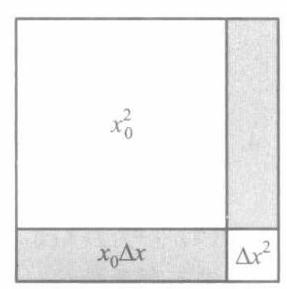
\includegraphics[width=.3\textwidth]{images/P029.jpg}
	\caption{图 $5-8$}
	\label{fig:P029}
\end{figure}

%定义  1
\begin{definition}{}{def:}
设函数 \(y = f\left( x\right)\) 定义在点 \({x}_{0}\) 的某邻域 \(U\left( {x}_{0}\right)\) 上. 当给 \({x}_{0}\) 一个增量 \({\Delta x},{x}_{0} + {\Delta x} \in  U\left( {x}_{0}\right)\) 时,相应地得到函数的增量为
\[
{\Delta y} = f\left( {{x}_{0} + {\Delta x}}\right)  - f\left( {x}_{0}\right) .
\]
如果存在常数 \(A\) ,使得 \({\Delta y}\) 能表示成
\[
{\Delta y} = {A\Delta x} + o\left( {\Delta x}\right) , \tag{1}
\]
则称函数 \(f\) 在点 \({x}_{0}\) 可微,并称 (1) 式中的第一项 \({A\Delta x}\) 为 \(f\) 在点 \({x}_{0}\) 的微分,记作
\[
{\left. \mathrm{d}y\right| }_{x = {x}_{0}} = {A\Delta x}\text{ 或 }{\left. \mathrm{d}f\left( x\right) \right| }_{x = {x}_{0}} = {A\Delta x}. \tag{2}
\]
\end{definition}

由定义可见,函数的微分与增量仅相差一个关于 \({\Delta x}\) 的高阶无穷小量,由于 \(\mathrm{d}y\) 是 \({\Delta x}\) 的线性函数,所以当 \(A \neq  0\) 时,也说微分 \(\mathrm{d}y\) 是增量 \({\Delta y}\) 的线性主部.

容易看出,函数 \(f\) 在点 \({x}_{0}\) 可导和可微是等价的.

%定理 5.9
\begin{theorem}{}{the:}
函数 \(f\) 在点 \({x}_{0}\) 可微的充要条件是函数 \(f\) 在点 \({x}_{0}\) 可导,而且 (1) 式中的 \(A\) 等于 \({f}^{\prime }\left( {x}_{0}\right)\) .
\end{theorem}


%证
\begin{proof}
必要性 若 \(f\) 在点 \({x}_{0}\) 可微,由 (1) 式有
\[
\frac{\Delta y}{\Delta x} = A + o\left( 1\right) .
\]
取极限后有
\[
{f}^{\prime }\left( {x}_{0}\right)  = \mathop{\lim }\limits_{{{\Delta x} \rightarrow  0}}\frac{\Delta y}{\Delta x} = \mathop{\lim }\limits_{{{\Delta x} \rightarrow  0}}\left\lbrack  {A + o\left( 1\right) }\right\rbrack   = A.
\]
这就证明了 \(f\) 在点 \({x}_{0}\) 可导且导数等于 \(A\) .

充分性 若 \(f\) 在点 \({x}_{0}\) 可导,则 \(f\) 在点 \({x}_{0}\) 的有限增量公式
\[
{\Delta y} = {f}^{\prime }\left( {x}_{0}\right) {\Delta x} + o\left( {\Delta x}\right)
\]
表明函数增量 \({\Delta y}\) 可表示为 \({\Delta x}\) 的线性部分 \(\left( {{f}^{\prime }\left( {x}_{0}\right) {\Delta x}}\right)\) 与较 \({\Delta x}\) 高阶的无穷小量之和, 所以 \(f\) 在点 \({x}_{0}\) 可微,且有
\[
{\left. \mathrm{d}y\right| }_{x = {x}_{0}} = {f}^{\prime }\left( {x}_{0}\right) {\Delta x}.
\]
\end{proof}

微分的几何解释如图 5-9 所示. 当自变量由 \({x}_{0}\) 增加到 \({x}_{0} + {\Delta x}\) 时,函数增量 \({\Delta y} =\)  \(f\left( {{x}_{0} + {\Delta x}}\right)  - f\left( {x}_{0}\right)  = {RQ}\) ,而微分则是在点 \(P\) 处的切线上与 \({\Delta x}\) 所对应的增量
\[
\mathrm{d}y = {f}^{\prime }\left( {x}_{0}\right) {\Delta x} = R{Q}^{\prime },
\]
\begin{figure}
	\centering
	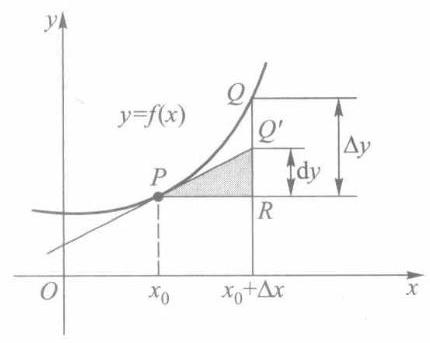
\includegraphics[width=.3\textwidth]{images/P030.jpg}
	\caption{图 $5-9$}
	\label{fig:P030}
\end{figure}

并且
\[
\mathop{\lim }\limits_{{x \rightarrow  {x}_{0}}}\frac{{\Delta y} - \mathrm{d}y}{\Delta x} = \mathop{\lim }\limits_{{x \rightarrow  {x}_{0}}}\frac{{Q}^{\prime }Q}{PR} = {f}^{\prime }\left( {x}_{0}\right) \mathop{\lim }\limits_{{x \rightarrow  {x}_{0}}}\frac{{Q}^{\prime }Q}{R{Q}^{\prime }} = 0,
\]
所以当 \({f}^{\prime }\left( {x}_{0}\right)  \neq  0\) 时,
\[
\mathop{\lim }\limits_{{x \rightarrow  {x}_{0}}}\frac{{Q}^{\prime }Q}{R{Q}^{\prime }} = 0.
\]
这表明当 \(x \rightarrow  {x}_{0}\) 时线段 \({Q}^{\prime }Q\) 的长度比 \(R{Q}^{\prime }\) 的长度要小得多.

若函数 \(y = f\left( x\right)\) 在区间上每一点都可微,则称 \(f\) 为 \(I\) 上的可微函数. 函数 \(y = f\left( x\right)\) 在 \(I\) 上任一点 \(x\) 处的微分记作
\[
\mathrm{d}y = {f}^{\prime }\left( x\right) {\Delta x},x \in  I, \tag{3}
\]
它不仅依赖于 \({\Delta x}\) ,而且也依赖于 \(x\) .

特别当 \(y = x\) 时,
\[
\mathrm{d}y = \mathrm{d}x = {\Delta x},
\]
这表示自变量的微分 \(\mathrm{d}x\) 就等于自变量的增量. 于是可将 (3) 式改写为
\[
\mathrm{d}y = {f}^{\prime }\left( x\right) \mathrm{d}x, \tag{4}
\]
即函数的微分等于函数的导数与自变量微分的积. 比如
\[
\mathrm{d}\left( {x}^{\alpha }\right)  = \alpha {x}^{\alpha  - 1}\mathrm{\;d}x,
\]
\[
\mathrm{d}\left( {\sin x}\right)  = \cos x\mathrm{\;d}x,
\]
\[
\mathrm{d}\left( {\ln x}\right)  = \frac{\mathrm{d}x}{x}.
\]
如果把 (4) 式写成
\[
{f}^{\prime }\left( x\right)  = \frac{\mathrm{d}y}{\mathrm{\;d}x},
\]
那么函数的导数就等于函数微分与自变量微分的商. 因此, 导数也常称为微商. 在这以前,我们总把 \(\frac{\mathrm{d}y}{\mathrm{\;d}x}\) 作为一个运算记号的整体来看待,有了微分概念之后,也不妨把它看作一个分式了.

\subsection{微分的运算法则}

由导数与微分的关系, 我们能立刻推出如下微分运算法则:

1. \(\mathrm{d}\left\lbrack  {u\left( x\right)  \pm  v\left( x\right) }\right\rbrack   = \mathrm{d}u\left( x\right)  \pm  \mathrm{d}v\left( x\right)\) ;

2. \(\mathrm{d}\left\lbrack  {u\left( x\right) v\left( x\right) }\right\rbrack   = v\left( x\right) \mathrm{d}u\left( x\right)  + u\left( x\right) \mathrm{d}v\left( x\right)\) ;

3. \(\mathrm{d}\left\lbrack  \frac{u\left( x\right) }{v\left( x\right) }\right\rbrack   = \frac{v\left( x\right) \mathrm{d}u\left( x\right)  - u\left( x\right) \mathrm{d}v\left( x\right) }{{v}^{2}\left( x\right) }\left( {v\left( x\right)  \neq  0}\right)\) ;

4. \(\mathrm{d}\left\lbrack  {f \circ  g\left( x\right) }\right\rbrack   = {f}^{\prime }\left( u\right) {g}^{\prime }\left( x\right) \mathrm{d}x\) ,其中 \(u = g\left( x\right)\) .

在上述复合函数的微分运算法则 4 中,由于 \(\mathrm{d}u = {g}^{\prime }\left( x\right) \mathrm{d}x\) ,所以它也可写作
\[
\mathrm{d}y = {f}^{\prime }\left( u\right) \mathrm{d}u.
\]
这与 (4) 式在形式上完全相同,即 (4) 式不仅在 \(x\) 为自变量时成立,当它是另一可微函数的因变量时也成立. 这个性质通常称为一阶微分形式的不变性.

%例 1
\begin{example}
求 \(y = {x}^{2}\ln x + \cos {x}^{2}\) 的微分.
\end{example}


%解
\begin{solution}
\(\mathrm{d}y = \mathrm{d}\left( {{x}^{2}\ln x + \cos {x}^{2}}\right)  = \mathrm{d}\left( {{x}^{2}\ln x}\right)  + \mathrm{d}\left( {\cos {x}^{2}}\right)\)
\[
= \ln x\mathrm{\;d}\left( {x}^{2}\right)  + {x}^{2}\mathrm{\;d}\left( {\ln x}\right)  + \mathrm{d}\left( {\cos {x}^{2}}\right)  = x\left( {2\ln x + 1 - 2\sin {x}^{2}}\right) \mathrm{d}x\text{ . }
\]
\end{solution}

%例 2
\begin{example}
求 \(y = {\mathrm{e}}^{\sin \left( {{ax} + b}\right) }\) 的微分.

\end{example}

%解
\begin{solution}
由一阶微分形式不变性, 可得
\[
\mathrm{d}y = {\mathrm{e}}^{\sin \left( {{ax} + b}\right) }\mathrm{d}\left\lbrack  {\sin \left( {{ax} + b}\right) }\right\rbrack
\]
\[
= {\mathrm{e}}^{\sin \left( {{ax} + b}\right) }\cos \left( {{ax} + b}\right) \mathrm{d}\left( {{ax} + b}\right)  = a{\mathrm{e}}^{\sin \left( {{ax} + b}\right) }\cos \left( {{ax} + b}\right) \mathrm{d}x. \tag{0}
\]
\end{solution}

\subsection{高阶微分}

我们知道函数 \(y = f\left( x\right)\) 的一阶微分是
\[
\mathrm{d}y = {f}^{\prime }\left( x\right) \mathrm{d}x,
\]
其中变量 \(x\) 和 \(\mathrm{d}x\) 是相互独立的. 现将一阶微分只作为 \(x\) 的函数,若 \(f\) 二阶可导,那么 \(\mathrm{d}y\) 对自变量 \(x\) 的微分
\[
\mathrm{d}\left( {\mathrm{d}y}\right)  = \mathrm{d}\left( {{f}^{\prime }\left( x\right) \mathrm{d}x}\right)  = {f}^{\prime \prime }\left( x\right) \mathrm{d}x \cdot  \mathrm{d}x = {f}^{\prime \prime }\left( x\right) {\left( \mathrm{d}x\right) }^{2},
\]
或写作
\[
{\mathrm{d}}^{2}y = {f}^{\prime \prime }\left( x\right) \mathrm{d}{x}^{2}, \tag{5}
\]
称它为函数 \(f\) 的二阶微分.

%注
\begin{remark}
这里 \(\mathrm{d}{x}^{2}\) 是指 \({\left( \mathrm{d}x\right) }^{2};{\mathrm{d}}^{2}x\) 表示 \(x\) 的二阶微分 \(\left( {{\mathrm{d}}^{2}x = 0}\right)\) ; 而 \(\mathrm{d}\left( {x}^{2}\right)\) 则表示 \({x}^{2}\) 的一阶微分 \(\left( {\mathrm{d}\left( {x}^{2}\right)  = {2x}\mathrm{\;d}x}\right)\) . 三者不能混淆.
\end{remark}


一般地, \(n\) 阶微分是 \(n - 1\) 阶微分的微分,记作 \({\mathrm{d}}^{n}y\) ,即
\[
{\mathrm{d}}^{n}y = \mathrm{d}\left( {{\mathrm{d}}^{n - 1}y}\right)  = \mathrm{d}\left( {{f}^{\left( n - 1\right) }\left( x\right) \mathrm{d}{x}^{n - 1}}\right)
\]
\[
= {f}^{\left( n\right) }\left( x\right) \mathrm{d}{x}^{n}.
\]
若将它写成
\[
\frac{{\mathrm{d}}^{n}y}{\mathrm{\;d}{x}^{n}} = {f}^{\left( n\right) }\left( x\right)
\]
时,就和 \(n\) 阶导数的记法一致了.

对 \(n \geq  2\) 的 \(n\) 阶微分均称为高阶微分.

一阶微分具有形式不变性, 而对于高阶微分来说已不具备这个性质了. 以二阶微分为例,当 \(x\) 为 \(y = f\left( x\right)\) 的自变量时,
\[
{\mathrm{d}}^{2}y = {f}^{\prime \prime }\left( x\right) \mathrm{d}{x}^{2}. \tag{6}
\]
当 \(x\) 为复合函数 \(y = f\left( x\right) ,x = \varphi \left( t\right)\) 的中间变量时, \(y = f\left( {\varphi \left( t\right) }\right)\) 作为 \(t\) 的函数,关于 \(t\) 的一阶微分可以写作
\[
\mathrm{d}y = {f}^{\prime }\left( x\right) \mathrm{d}x,
\]
其中 \(\mathrm{d}x = {\varphi }^{\prime }\left( t\right) \mathrm{d}t\) ; 而对 \(t\) 的二阶微分则为
\[
{\mathrm{d}}^{2}y = {\left( f\left( \varphi \left( t\right) \right) \right) }^{\prime \prime }\mathrm{d}{t}^{2} = {\left( {f}^{\prime }\left( \varphi \left( t\right) \right) {\varphi }^{\prime }\left( t\right) \right) }^{\prime }\mathrm{d}{t}^{2}
\]
\[
= \left\lbrack  {{f}^{\prime \prime }\left( {\varphi \left( t\right) }\right) {\left( {\varphi }^{\prime }\left( t\right) \right) }^{2} + {f}^{\prime }\left( {\varphi \left( t\right) }\right) {\varphi }^{\prime \prime }\left( t\right) }\right\rbrack  \mathrm{d}{t}^{2}
\]
\[
= {f}^{\prime \prime }\left( x\right) \mathrm{d}{x}^{2} + {f}^{\prime }\left( x\right) {\mathrm{d}}^{2}x, \tag{7}
\]
它比 (5) 式多了一项, 这说明二阶微分已不再具有形式不变性.

%例 3
\begin{example}
设 \(y = f\left( x\right)  = \sin x,x = \varphi \left( t\right)  = {t}^{2}\) . 分别依公式 (6) 和公式 (7) 求 \({\mathrm{d}}^{2}y\) .
\end{example}


%解
\begin{solution}
由 \(y = \sin {t}^{2}\) 得 \({y}^{\prime } = {2t}\cos {t}^{2},{y}^{\prime \prime } = 2\cos {t}^{2} - 4{t}^{2}\sin {t}^{2}\) ,依公式 (6) 得
\[
{\mathrm{d}}^{2}y = \left( {2\cos {t}^{2} - 4{t}^{2}\sin {t}^{2}}\right) \mathrm{d}{t}^{2}.
\]
类似地, 依公式 (7) 可得
\[
{\mathrm{d}}^{2}y = {f}^{\prime \prime }\left( x\right) \mathrm{d}{x}^{2} + {f}^{\prime }\left( x\right) {\mathrm{d}}^{2}x
\]
\[
=  - \sin x\mathrm{\;d}{x}^{2} + \cos x{\mathrm{\;d}}^{2}x
\]
\[
=  - \sin {t}^{2} \cdot  {\left( 2t\right) }^{2}\mathrm{\;d}{t}^{2} + \cos {t}^{2} \cdot  2\mathrm{\;d}{t}^{2}
\]
\[
= \left( {2\cos {t}^{2} - 4{t}^{2}\sin {t}^{2}}\right) \mathrm{d}{t}^{2}\text{ . }
\]
\end{solution}

%注
\begin{remark}
下面的解法是错误的:
\[
{\mathrm{d}}^{2}y = {f}^{\prime \prime }\left( x\right) \mathrm{d}{x}^{2} =  - \sin x{\left( 2t\mathrm{\;d}t\right) }^{2} =  - 4{t}^{2}\sin {t}^{2}\mathrm{\;d}{t}^{2}.
\]
\end{remark}

\subsection{微分在近似计算中的应用}

微分在数学中有许多重要的应用. 这里介绍它在近似计算方面的一些应用.

1. 函数的近似计算 由函数增量与微分关系
\[
{\Delta y} = {f}^{\prime }\left( {x}_{0}\right) {\Delta x} + o\left( {\Delta x}\right)  = \mathrm{d}y + o\left( {\Delta x}\right) ,
\]
当 \({\Delta x}\) 很小时,有 \({\Delta y} \approx  \mathrm{d}y\) ,由此即得
\[
f\left( {{x}_{0} + {\Delta x}}\right)  \approx  f\left( {x}_{0}\right)  + {f}^{\prime }\left( {x}_{0}\right) {\Delta x}, \tag{8}
\]
或当 \(x \approx  {x}_{0}\) 时有
\[
f\left( x\right)  \approx  f\left( {x}_{0}\right)  + {f}^{\prime }\left( {x}_{0}\right) \left( {x - {x}_{0}}\right) . \tag{9}
\]
注意到在点 \(\left( {{x}_{0},f\left( {x}_{0}\right) }\right)\) 的切线方程即为
\[
y = f\left( {x}_{0}\right)  + {f}^{\prime }\left( {x}_{0}\right) \left( {x - {x}_{0}}\right) ,
\]
(9)式的几何意义就是当 \(x\) 充分接近 \({x}_{0}\) 时,可用切线近似替代曲线 (以直代曲). 常用这种线性近似的思想来对复杂问题进行简化处理.

设 \(f\left( x\right)\) 分别是 \(\sin x,\tan x,\ln \left( {1 + x}\right)\) 和 \({\mathrm{e}}^{x}\) ,令 \({x}_{0} = 0\) ,则由 (9) 式可得这些函数在原点附近的近似公式:
\[
\sin x \approx  x,\;\tan x \approx  x,
\]
\[
\ln \left( {1 + x}\right)  \approx  x,\;{\mathrm{e}}^{x} \approx  1 + x.
\]
一般地,为求得 \(f\left( x\right)\) 的近似值,可找一邻近于 \(x\) 的点 \({x}_{0}\) ,只要 \(f\left( {x}_{0}\right)\) 和 \({f}^{\prime }\left( {x}_{0}\right)\) 易于计算,由 (9) 式可求得 \(f\left( x\right)\) 的近似值.

%例 4
\begin{example}
求 \(\sin {33}^{ \circ  }\) 的近似值.
\end{example}


%解
\begin{solution}
由于 \(\sin {33}^{ \circ  } = \sin \left( {\frac{\pi }{6} + \frac{\pi }{60}}\right)\) ,因此取 \(f\left( x\right)  = \sin x,{x}_{0} = \frac{\pi }{6},{\Delta x} = \frac{\pi }{60}\) ,由 (9) 式得到
\[
\sin {33}^{ \circ  } \approx  \sin \frac{\pi }{6} + \cos \frac{\pi }{6} \cdot  \frac{\pi }{60} = \frac{1}{2} + \frac{\sqrt{3}}{2} \cdot  \frac{\pi }{60} \approx  {0.545}.
\]
\(\left( {\sin {33}^{ \circ  }}\right.\) 的真值为 \({0.544639}\cdots .)\)
\end{solution}


%例 5
\begin{example}
设钟摆的周期是 \(1\mathrm{\;s}\) ,在冬季摆长至多缩短 \({0.01}\mathrm{\;{cm}}\) ,试问此钟每天至多快几秒?
\end{example}


%解
\begin{solution}
由物理学知道,单摆周期 \(T\) 与摆长 \(l\) 的关系为
\[
T = {2\pi }\sqrt{\frac{l}{g}},
\]
其中 \(g\) 是重力加速度. 已知钟摆周期为 \(1\mathrm{\;s}\) ,故此摆原长为
\[
{l}_{0} = \frac{g}{{\left( 2\pi \right) }^{2}}.
\]
当摆长最多缩短 \({0.01}\mathrm{\;{cm}}\) 时,摆长的增量 \({\Delta l} =  - {0.01}\) ,它引起单摆周期的增量
\[
{\Delta T} \approx  {\left. \frac{\mathrm{d}T}{\mathrm{\;d}l}\right| }_{l = {l}_{0}} \cdot  {\Delta l} = \frac{\pi }{\sqrt{g}} \cdot  \frac{1}{\sqrt{{l}_{0}}}{\Delta l} = \frac{2{\pi }^{2}}{g}{\Delta l}
\]
\[
= \frac{2{\pi }^{2}}{980} \times  \left( {-{0.01}}\right)  \approx   - {0.0002}\left( \mathrm{\;s}\right) .
\]
这就是说,加快约 \({0.0002}\mathrm{\;s}\) ,因此每天大约加快
\[
{60} \times  {60} \times  {24} \times  {0.0002} = {17.28}\left( \mathrm{\;s}\right) .
\]
\end{solution}

2. 误差估计 设量 \(x\) 由测量得到,量 \(y\) 由函数 \(y = f\left( x\right)\) 经过计算得到. 在测量时,由于存在测量误差,实际测得的只是 \(x\) 的某一近似值 \({x}_{0}\) ,因此由 \({x}_{0}\) 算得的 \({y}_{0} = f\left( {x}_{0}\right)\) 也只是 \(y = f\left( x\right)\) 的一个近似值. 若已知测量值 \({x}_{0}\) 的误差限为 \({\delta }_{x}\) (它与测量工具的精度有关),即
\[
\left| {\Delta x}\right|  = \left| {x - {x}_{0}}\right|  \leq  {\delta }_{x},
\]
则当 \({\delta }_{x}\) 很小时,
\[
\left| {\Delta y}\right|  = \left| {f\left( x\right)  - f\left( {x}_{0}\right) }\right|  \approx  \left| {{f}^{\prime }\left( {x}_{0}\right) {\Delta x}}\right|  \leq  \left| {{f}^{\prime }\left( {x}_{0}\right) }\right| {\delta }_{x}, \tag{10}
\]
而相对误差限则为
\[
\frac{{\delta }_{y}}{\left| {y}_{0}\right| } = \left| \frac{{f}^{\prime }\left( {x}_{0}\right) }{f\left( {x}_{0}\right) }\right| {\delta }_{x}. \tag{11}
\]

%例 6
\begin{example}
设测得一球体的直径为 \({42}\mathrm{\;{cm}}\) ,测量工具的精度为 \({0.05}\mathrm{\;{cm}}\) . 试求以此直径计算球体体积时所引起的误差.

\end{example}

%解
\begin{solution}
由直径 \(d\) 计算球体体积的函数式为
\[
V = \frac{1}{6}\pi {d}^{3}.
\]
取 \({d}_{0} = {42},{\delta }_{d} = {0.05}\) ,求得
\[
{V}_{0} = \frac{1}{6}\pi {d}_{0}^{3} \approx  {38792.39}\left( {\mathrm{\;{cm}}}^{3}\right) ,
\]
并由 (10)、(11) 两式得体积的绝对误差限和相对误差限分别为
\[
{\delta }_{V} = \left| {\frac{1}{2}\pi {d}_{0}^{2}}\right|  \cdot  {\delta }_{d} = \frac{\pi }{2} \cdot  {42}^{2} \cdot  {0.05} \approx  {138.54}\left( {\mathrm{\;{cm}}}^{3}\right) ,
\]
\[
\frac{{\delta }_{V}}{\left| {V}_{0}\right| } = \frac{\frac{1}{2}\pi {d}_{0}^{2}}{\frac{1}{6}\pi {d}_{0}^{3}} \cdot  {\delta }_{d} = \frac{3}{{d}_{0}}{\delta }_{d} \approx  {3.57}\% \text{ . }
\]
\end{solution}

\subsection{习题 5.5}

1. 若 \(x = 1\) ,而 \({\Delta x} = {0.1},{0.01}\) . 问对于 \(y = {x}^{2},{\Delta y}\) 与 \(\mathrm{d}y\) 之差分别是多少?

2. 求下列函数的微分:

(1) \(y = x + 2{x}^{2} - \frac{1}{3}{x}^{3} + {x}^{4}\) ;

(2) \(y = x\ln x - x\) ;

(3) \(y = {x}^{2}\cos {2x}\) ;

(4) \(y = \frac{x}{1 - {x}^{2}}\) ;

(5) \(y = {\mathrm{e}}^{ax}\sin {bx}\) ;

(6) \(y = \arcsin \sqrt{1 - {x}^{2}}\) .

3. 求下列函数的高阶微分:

(1)设 \(u\left( x\right)  = \ln x,v\left( x\right)  = {\mathrm{e}}^{x}\) ,求 \({\mathrm{d}}^{3}\left( {uv}\right) ,{\mathrm{d}}^{3}\left( \frac{u}{v}\right)\) ；

(2)设 \(u\left( x\right)  = {\mathrm{e}}^{\frac{x}{2}},v\left( x\right)  = \cos {2x}\) ,求 \({\mathrm{d}}^{3}\left( {uv}\right) ,{\mathrm{d}}^{3}\left( \frac{u}{v}\right)\) .

4. 利用微分求近似值:

(1) \(\sqrt[3]{1.02}\) ;

(2) \(\lg {2.7}\) ;

(3) tan \({45}^{ \circ  }{10}^{\prime }\) ;

(4) \(\sqrt{26}\) .

5. 为了使计算出球的体积准确到 \(1\%\) ,问度量半径为 \(r\) 时允许发生的相对误差至多应为多少?

6. 检验一个半径为 \(2\mathrm{\;m}\) ,中心角为 \({55}^{ \circ  }\) 的工件面积 (图 5-10),现可直接测量其中心角或此角所对的弦长,设量角最大误差为 \({0.5}^{ \circ  }\) ,量弦长最大误差为 \(3\mathrm{\;{mm}}\) ,试问用哪一种方法检验的结果较为精确.


\begin{figure}
    \centering
    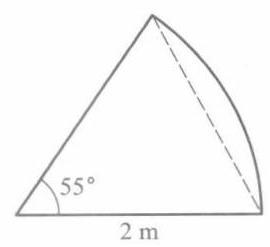
\includegraphics[width=.3\textwidth]{images/P031.jpg}
    \caption{图 $5-10$}
    \label{fig:P031}
\end{figure}

\section{第五章总练习题}

1. 设 \(y = \frac{{ax} + b}{{cx} + d}\) ,证明:

(1) \({y}^{\prime } = \frac{1}{{\left( cx + d\right) }^{2}}\left| \begin{array}{ll} a & b \\  c & d \end{array}\right|\) ;

(2) \({y}^{\left( n\right) } = {\left( -1\right) }^{n + 1}\frac{n!{c}^{n - 1}}{{\left( cx + d\right) }^{n + 1}}\left| \begin{matrix} a & b \\  c & d \end{matrix}\right|\) .

2. 证明下列函数在 \(x = 0\) 处不可导: (1) \(f\left( x\right)  = {x}^{\frac{2}{3}}\) ;

(2) \(f\left( x\right)  = \left| {\ln \left| {x - 1}\right| }\right|\) . 3. (1) 举出一个连续函数,它仅在已知点 \({a}_{1},{a}_{2},\cdots ,{a}_{n}\) 不可导; (2)举出一个函数,它仅在点 \({a}_{1},{a}_{2},\cdots ,{a}_{n}\) 可导.

4. 证明: (1)可导的偶函数,其导函数为奇函数； (2)可导的奇函数,其导函数为偶函数； (3)可导的周期函数,其导函数仍为周期函数.

5. 对下列命题,若认为是正确的,请给予证明；若认为是错误的,请举一反例予以否定:

(1) 设 \(f = \varphi  + \psi\) ,若 \(f\) 在点 \({x}_{0}\) 可导,则 \(\varphi ,\psi\) 在点 \({x}_{0}\) 可导;

(2)设 \(f = \varphi  + \psi\) ,若 \(\varphi\) 在点 \({x}_{0}\) 可导, \(\psi\) 在点 \({x}_{0}\) 不可导,则 \(f\) 在点 \({x}_{0}\) 一定不可导；

(3) 设 \(f = \varphi  \cdot  \psi\) ,若 \(f\) 在点 \({x}_{0}\) 可导,则 \(\varphi ,\psi\) 在点 \({x}_{0}\) 可导;

(4)设 \(f = \varphi  \cdot  \psi\) ,若 \(\varphi\) 在点 \({x}_{0}\) 可导, \(\psi\) 在点 \({x}_{0}\) 不可导,则 \(f\) 在点 \({x}_{0}\) 一定不可导.

6. 设 \(\varphi \left( x\right)\) 在点 \(a\) 连续, \(f\left( x\right)  = \left| {x - a}\right| \varphi \left( x\right)\) ,求 \({f}_{ - }^{\prime }\left( a\right)\) 和 \({f}_{ + }^{\prime }\left( a\right)\) . 问在什么条件下 \({f}^{\prime }\left( a\right)\) 存在?

7. 设 \(f\) 为可导函数,求下列各函数的一阶导数:

(1) \(y = f\left( {\mathrm{e}}^{x}\right) {\mathrm{e}}^{f\left( x\right) }\) ;

(2) \(y = f\left( {f\left( {f\left( x\right) }\right) }\right)\) ).

8. 设 \(\varphi ,\psi\) 为可导函数,求 \({y}^{\prime }\) :

(1) \(y = \sqrt{{\left\lbrack  \varphi \left( x\right) \right\rbrack  }^{2} + {\left\lbrack  \psi \left( x\right) \right\rbrack  }^{2}}\) ;

(2) \(y = \arctan \frac{\varphi \left( x\right) }{\psi \left( x\right) }\) ;

(3) \(y = {\log }_{\varphi \left( x\right) }\psi \left( x\right) \left( {\varphi ,\psi  > 0,\varphi  \neq  1}\right)\) .

9. 设 \({f}_{ij}\left( x\right) \left( {i,j = 1,2,\cdots ,n}\right)\) 为可导函数,证明:
\[
\frac{\mathrm{d}}{\mathrm{d}x}\left| \begin{matrix} {f}_{11}\left( x\right) & {f}_{12}\left( x\right) & \cdots & {f}_{1n}\left( x\right) \\  {f}_{21}\left( x\right) & {f}_{22}\left( x\right) & \cdots & {f}_{2n}\left( x\right) \\  \vdots & \vdots & & \vdots \\  {f}_{n1}\left( x\right) & {f}_{n2}\left( x\right) & \cdots & {f}_{nn}\left( x\right)  \end{matrix}\right|  = \mathop{\sum }\limits_{{k = 1}}^{n}\left| \begin{matrix} {f}_{11}\left( x\right) & {f}_{12}\left( x\right) & \cdots & {f}_{1n}\left( x\right) \\  {f}_{21}\left( x\right) & {f}_{22}\left( x\right) & \cdots & {f}_{2n}\left( x\right) \\  \vdots & \vdots & & \vdots \\  {f}_{k1}^{\prime }\left( x\right) & {f}_{k2}^{\prime }\left( x\right) & \cdots & {f}_{kn}^{\prime }\left( x\right) \\  \vdots & \vdots & & \vdots \\  {f}_{n1}\left( x\right) & {f}_{n2}^{\prime }\left( x\right) & \cdots & {f}_{nn}^{\prime }\left( x\right)  \end{matrix}\right| .
\]
并利用这个结果求 \({F}^{\prime }\left( x\right)\) :

(1) \(F\left( x\right)  = \left| \begin{matrix} x - 1 & 1 & 2 \\   - 3 & x & 3 \\   - 2 &  - 3 & x + 1 \end{matrix}\right|\) ;

(2) \(F\left( x\right)  = \left| \begin{matrix} x & {x}^{2} & {x}^{3} \\  1 & {2x} & 3{x}^{2} \\  0 & 2 & {6x} \end{matrix}\right|\) .

\subsection{第五章综合自测题}

